\chapter{Introduction}
 
The use of logic has always had an important place in various sciences,
especially in computer science and, in particular, formal verification. The
expressiveness of logics allows to specify verified systems in a very natural
and intuitive way without the need of deep knowledge of the used verification
procedures. The logic used range from plain propositional logic through all
kinds of first-order logics like Presburger arithmetic \cite{presburger},
separation logic, and all the way to the more complex monadic second-order
logics, like WS$k$S \cite{wsks}. However, with great expressiveness comes great
complexity of decision problems of these logics, ranging from NP-complete for
propositional logic, through PSPACE-complete for quantified Boolean formulae,
with some stronger logics not being decidable at all.

WS$k$S stands for \emph{weak monadic second-order logic of $k$ successors}.
Roughly, this means that it allows to quantify over finite set variables where
every element from the universe of discourse has $k$ successors. This properties
open ways for expressing various $k$-ary tree structures, e.g. binary trees or
heaps, and linear structures, e.g. linked lists, as well. Decision procedures
for WS$k$S are usually based on the correspondence between WS$k$S formulae and
languages of finite automata (be it word or tree automata). The atomic
subformulae of an
examined WS$k$S formula $\phi$ are translated to finite (word/tree)
automata, which are further connected or manipulated using automata manipulation
techniques according to the structure of $\phi$. The resulting automaton then
represents the language encoding all models of $\phi$. The problem of checking
satisfiability or unsatisfiability/validity/invalidity of $\phi$ is in the
NONELEMENTARY complexity class.

There has been several attempts to implement a~decision procedure for WS$k$S,
like~\cite{nfa} for $k = 1$. Currently the best one is the tool \textsc{MONA}
\cite{mona}, an implementation of an automata-based decision procedure which is
quite fast and uses deterministic finite word and binary bottom-up tree automata
for deciding WS1S and WS2S formulae respectively. The authors of \textsc{MONA}
have developed a number of heuristics, such as the use of binary decision
diagrams for the representation of transition functions of automata or
cache-friendly implementation of hash tables that made \textsc{MONA} perform
well on many practical examples in spite of the terrifying worst-case
complexity.

Recently, there has been a major advance in the algorithms manipulating
non-deter\-mi\-ni\-stic automata (like \cite{vata}). Even problems with high
worst-case complexity like testing universality or language inclusion of
automaton, can now be solved efficiently in many practical cases using
algorithms that heuristically prune the search space, such as algorithms based
on antichains or on the simulation relation among states of automata.

The main goal of this work is the design and implementation of a decision
procedure for WS$k$S that uses non-deterministic tree automata while exploiting
the techniques for their efficient manipulation to achieve better performance.

The rest of this thesis is organized as follows. In Chapter \ref{preli} all
necessary preliminaries are defined. A~short introduction to the theory of
formal languages will describe finite word and tree automata, as well as some
properties of their languages. Another structure that will be defined there will
be Binary Decision Diagrams, or BDDs for short, and their extensions. Chapter
\ref{wsks} defines the syntax and semantics of the WS$k$S logic and its restricted
forms. A Brief description of the correspondence between tree automata and
WS$k$S formulae also appears there.
Chapter \ref{monachap} describes the approach of \textsc{MONA} and all the
tweaks and secrets that were discovered during its development. In Chapter
\ref{our} our approach to  a decision procedure for the WS$k$S logic using
non-deterministic automata and its anti-chain based principle will be outlined.
A~short introduction to antichain-based procedures and universality testing of
finite word and tree automata is described there as well. Chapter \ref{summary}
summarizes this thesis.

\chapter{Preliminaries}\label{preli}

 \section{Formal Languages}

 We define an \emph{alphabet} as a finite non-empty set of elements called
 \emph{symbols}. A~\emph{word} over the alphabet $\Sigma$ is a finite sequence
 $a_1a_2\ldots a_n$, such that $a_i \in \Sigma$, for all $1 \leq i \leq n$. The
 \emph{empty sequence} of symbols, i.e. a sequence  which does not contain any
 symbols, is denoted as $\epsilon$.

Let $x = a_1a_2\ldots a_n$ and $y = b_1b_2\ldots b_m$ be words over the alphabet
$\Sigma$, for some $n, m \in \mathbb{N}$. The \emph{concatenation} of words $x$
and $y$ is defined as the word $xy = a_1a_2\ldots a_nb_1b_2\ldots b_m$. Note
that $\epsilon x = x \epsilon = x$.

Let $\Sigma$ be an alphabet. We denote the set of all words over $\Sigma$ as
$\Sigma^*$. The set of all words except for the empty word is denoted as
$\Sigma^+ = \Sigma^* \setminus \{\epsilon\}$. We call $L \subseteq \Sigma^*$ the
language over $\Sigma$.

 \section{Finite Automata}

 A~\emph{non-deterministic finite} (word) \emph{automaton} (further abbreviated
 as FA) is a quintuple $\mathcal{A} = (Q, \Sigma, \delta, I, F)$, where
  \begin{itemize}
\item $Q$ is a finite set of \emph{states}, \item $I$ $ \subseteq Q$ is the set
of \emph{initial states}, \item $F$ $ \subseteq Q$ is the set of \emph{final
states}, \item $\Sigma$ is the input alphabet, \item $\delta$ $ \subseteq Q
\times\Sigma\times Q$ is the transition relation. We use $p
\overset{a}{\longrightarrow} q$, for $p, q \in Q$ and $a \in \Sigma$ to denote
that $(p, a, q) \in \delta$.
	\end{itemize}
	
Let $\mathcal{A} = (Q, \Sigma, \delta, I, F)$ be a FA. A~\emph{run} of
$\mathcal{A}$ over the word $w = a_1a_2\ldots a_n \in \Sigma^*$ from the state
$p \in Q$ to the state $r \in Q$ is a sequence of states $q_0q_1\ldots q_n$,
such that $q_0 = p, q_n = r$ and for all $1 \leq i \leq n$ there is a transition
$q_{i-1} \overset{a_i}{\longrightarrow} q_i$ in $\delta$. We write $p
\overset{w}{\Longrightarrow} r$ to denote that there exists a~run from the state
$p$ to the state $r$ over the word $w$.
	
The \emph{language} accepted by a state $q \in Q$ is defined as
$L_{\mathcal{A}}(q) = \{w \mid q \overset{w}{\Longrightarrow} q_f, q_f \in F\}$.
If it is clear which FA $\mathcal{A}$ we are referring to, we can simplify
this to $L(q)$. The language accepted by a set of states $S \subseteq
Q$ is further defined as $L_{\mathcal{A}}(S) = \bigcup_{q \in S}
L_{\mathcal{A}}(q)$ and the language accepted by the automaton $\mathcal{A}$ is
defined as $L(\mathcal{A}) = L_{\mathcal{A}}(I)$.
	
A~\emph{deterministic finite automaton} (DFA) is a FA $\mathcal{A}$ where $|I| =
1$ and $\forall q \in Q, \forall a \in \Sigma: |\{ r \in Q \mid q
\overset{a}{\longrightarrow} r\}| \leq 1$, i.e. $\delta$ is a partial function
$\delta : Q \times \Sigma \longrightarrow Q$. If $\delta$ is total, i.e.
$\forall q \in Q, \forall a \in \Sigma : |\delta(q, a)| = 1$, we call
$\mathcal{A}$ a \emph{complete deterministic finite automaton}. It can be shown
that for every deterministic FA there exists a language equivalent complete
deterministic FA, by adding a new non-final sink state.
	
	\begin{lemma}
For every non-deterministic finite automata $\mathcal{A}$, there exists a
deterministic finite automata $\mathcal{A}'$ such that $L(\mathcal{A}) =
L(\mathcal{A}')$.
	\end{lemma}
	
	\begin{proof}
	Let $\mathcal{A} = (Q, \Sigma, \delta, I, F)$ be a FA. We can construct
	the DFA $\mathcal{A}'= (Q', \Sigma, \delta', I', F')$, such that
	$L(\mathcal{A}) = L(\mathcal{A}')$, by the following method:
	\begin{eqnarray*}
	 Q' & = & 2^Q\\
	 I' & = & \{I\}\\
	 F' & = & \{S \in 2^Q \mid S~\cap F \neq \emptyset\}\\
	 \delta'(S, a) & = & \{r \in Q \mid q \overset{a}{\longrightarrow} r \in
	 \delta\}
	\end{eqnarray*}
	
	Note that $\mathcal{A}'$ is complete.
	
	It can be proved that $L(\mathcal{A}) = L(\mathcal{A}')$ by showing that
	$L(\mathcal{A}) \subseteq L(\mathcal{A}')$ and simultaneously $L(\mathcal{A}')
	\subseteq L(\mathcal{A})$ \cite{tin}.
	\end{proof}
	
	\begin{defz}
We define the class of regular languages $\mathcal{L}_R$ as the class of
languages $L \in \Sigma^*$ such that there exists a finite automata
$\mathcal{A}$ such that $L(\mathcal{A}) = L$.
	\end{defz}
	
	\noindent\hrulefill
	\begin{example}
	Consider coding of subsets of $\{1,\ldots,n\}$, for some $n \in \mathbb{N}$, as
	binary strings $X = a_1\ldots a_n$, where $a_i$ is $1$ if $i \in X$ and $0$ if
	$i \notin X$.
	
	We can construct automaton $\mathcal{A}$ that accepts set difference $X$ of two
	sets $Y$ and $Z$, i.e. $X = Y \setminus Z$, as depicted in Figure
	\ref{set-automaton}.
	
	\begin{figure}[h!]
	\begin{center}
	 \scalebox{1}{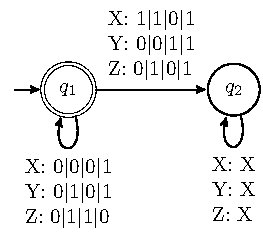
\includegraphics{fig/word-automaton-setminus.pdf}}
	 \end{center}
	 \caption{Automaton $\mathcal{A}$ accepting set difference of two
	 sets.}\label{set-automaton}
	\end{figure}
	\end{example}
	
	\noindent\hrulefill
	
 \subsection{Closure Properties of Regular Languages}

\begin{theorem}
 The class of regular languages is closed under union.
\end{theorem}

\begin{proof}
Let $\mathcal{A} = (Q_\mathcal{A}, \Sigma, \delta_\mathcal{A}, I_\mathcal{A},
F_\mathcal{A})$ and $\mathcal{B} = (Q_\mathcal{B}, \Sigma, \delta_\mathcal{B},
I_\mathcal{B}, F_\mathcal{B})$ be a pair of finite automata such that
$Q_\mathcal{A} \cap Q_\mathcal{B}$. We construct an automaton accepting the
\emph{union} of languages $L(\mathcal{A})$ and $L(\mathcal{B})$  
 \begin{equation} \mathcal{A} \cup \mathcal{B} = (Q_\mathcal{A} \cup
 Q_\mathcal{B}, \Sigma, \delta_\mathcal{A} \cup \delta_\mathcal{B},
 I_\mathcal{A} \cup I_\mathcal{B}, F_\mathcal{A} \cup
F_\mathcal{B})
\end{equation}
	
The roof that $L(\mathcal{A} \cup \mathcal{B}) = L(\mathcal{A}) \cup
L(\mathcal{B})$ can be found for example in \cite{tin}.
\end{proof}

  \begin{theorem}
	 The class of regular languages is closed under intersection.
	\end{theorem}
	
	\begin{proof}
Let $\mathcal{A} = (Q_\mathcal{A}, \Sigma, \delta_\mathcal{A}, I_\mathcal{A},
F_\mathcal{A})$ and $\mathcal{B} = (Q_\mathcal{B}, \Sigma, \delta_\mathcal{B},
I_\mathcal{B}, F_\mathcal{B})$ be a pair of finite automata. We construct an
automaton accepting the \emph{intersection} of languages $L(\mathcal{A})$ and
$L(\mathcal{B})$ 
\begin{equation}
\mathcal{A} \cap \mathcal{B} = (Q_\mathcal{A} \times
Q_\mathcal{B}, \Sigma, \delta, I_\mathcal{A} \times I_\mathcal{B}, F_\mathcal{A}
\times F_\mathcal{B})
\end{equation} where 
\begin{equation}
\delta = \{(p_1, p_2)
\overset{a}{\longrightarrow} (q_1, q_2) \mid (p_1, a, q_1) \in \delta_\mathcal{A}
\wedge (p_2, a, q_2) \in \delta_\mathcal{B}\}
\end{equation}
	
The proof that $L(\mathcal{A} \cap \mathcal{B}) = L(\mathcal{A}) \cap
L(\mathcal{B})$ can be found for example in \cite{tin}.
\end{proof}
	
 \begin{theorem}
  The class of regular languages is closed under language complementation.
\end{theorem}
	
	\begin{proof}
Let $\mathcal{A} = (Q_\mathcal{A}, \Sigma, \delta_\mathcal{A}, I_\mathcal{A},
F_\mathcal{A})$ be a complete deterministic FA. We construct an automaton
accepting the \emph{complement} of $L(\mathcal{A})$ 
\begin{equation}
\overline{\mathcal{A}} =
(Q_\mathcal{A}, \Sigma, \delta_\mathcal{A}, I_\mathcal{A}, Q_\mathcal{A}
\setminus F_\mathcal{A})
\end{equation}
	
The proof that $L(\overline{\mathcal{A}}) = \Sigma^* \setminus L(\mathcal{A})$
can be found for example in \cite{tin}.
 \end{proof}

 \section{Tree Automata}

 A~\emph{ranked alphabet} $\Sigma$ is a finite set of symbols together with a
 ranking function $\#: \Sigma \to \mathbb{N}$, we call $\#a$ the \emph{rank}
 of $a$. For any $n \geq 0$, we denote by $\Sigma_n$ the set of all symbols of rank
 $n$ from $\Sigma$. We denote $\epsilon \in \mathbb{N}^*$ the \emph{empty
 sequence}.

Then a \emph{tree} $t$ over a ranked alphabet $\Sigma$ is defined as a partial
mapping $t : \mathbb{N}^* \to \Sigma$, that satisfies the following conditions:
 \begin{enumerate}
  \item \emph{dom}($t$) is a finite prefix-closed subset of $\mathbb{N}^*$,
  \item for every $v \in dom(t)$, called a \emph{node} of $t$, the following
holds: $(\#t(v) = n \geq 0) \Longrightarrow \{i \mid vi \in dom(t)\} =
\{1,\ldots,n\}$.
 \end{enumerate}

For a node $v$, the $i$-th \emph{child} of $v$ is the node $vi$, and the $i$-th
\emph{subtree} of $v$ is the tree $t'$ such that for all $v' \in \mathbb{N}^*$, 
$t'(v') = t(viv')$. A~node $v$ which does not have any children is called a
\emph{leaf} of the tree $t$. The set of all trees over the alphabet $\Sigma$ is
denoted as $T_\Sigma$.

A~(finite, non-deterministic) \emph{tree automaton} (further abbreviated as TA)
is a quadruple $\mathcal{A} = (Q, \Sigma, \delta, F)$, where:
 \begin{itemize}
   \item $Q$ is a finite set of \emph{states},
	\item $\Sigma$ is a \emph{ranked alphabet},
	\item $\delta$ is the \emph{set of transitions}.
	\item $F$ $ \subseteq Q$ is the set of \emph{final states},
 \end{itemize}

Each transition is defined as a triple $((q_1,\ldots,q_n), a, q)$, where
$q_1,\ldots,q_n,q \in Q, a \in \Sigma$ and $\#a = n$. We use equivalently
$(q_1,\ldots,q_n) \overset{a}{\longrightarrow} q$ and $q
\overset{a}{\longrightarrow}  (q_1,\ldots,q_n)$ to denote that
$((q_1,\ldots,q_n), a, q) \in \delta$, for \emph{bottom-up} and \emph{top-down}
representation respectively. In the special case where $n = 0$, we speak about
the so-called \emph{leaf rules} that can be abbreviated as
$\overset{a}{\longrightarrow}  q$ or $q \overset{a}{\longrightarrow} $.

Let $\mathcal{A} = (Q, \Sigma, \delta, F)$ be a TA. We define a \emph{run} of
$\mathcal{A}$ over a tree $t \in T_\Sigma$ as a mapping $\varphi: dom(t) \to Q$
such that for each node $v \in dom(t)$ of rank $\#t(v) = n$, where $\varphi(v) =
q$, if $\varphi(vi) = q_i$ for all $1 \leq i \leq n$, then $(q_1,\ldots,q_n)
\overset{t(v)}{\longrightarrow} q$. We write $t
\overset{\varphi}{\Longrightarrow} q$ to denote that $\varphi$ is a~run of
$\mathcal{A}$ over $t$ such that $\varphi(\epsilon) = q$. We will write $t
\Longrightarrow q$ to denote that there exists a run $\varphi$ for which $t
\overset{\varphi}{\Longrightarrow} q$.

The \emph{language} accepted by a state $q$ is defined as $L_{\mathcal{A}}(q) =
\{t \mid t \Rightarrow q\}$. For a set of states $S \subseteq Q$ we define the
language accepted by this set as $L_{\mathcal{A}}(S) = \bigcup_{q \in S}
L_{\mathcal{A}}(q)$. Similarly to FA, if it is clear which TA $\mathcal{A}$ we
are referring to, we only write $L(q)$ or $L(S)$. Then language of $\mathcal{A}$
is defined as $L(\mathcal{A}) = L(F)$.

\begin{defz}
A~\emph{deterministic finite tree automaton} (abbreviated as DTA) is a
TA such that there are no two rules with the
same left-hand, or right-hand, side in $\delta$ for bottom-up TA or top-down
TA respectively.
\end{defz}

Note that the expressive power of bottom-up and top-down NTA is the same.
However, top-down DTA are strictly less powerful than top-down NTA. See
\cite{tata} for more details.

\begin{defz}
We define the class of regular tree languages $\mathcal{L}$ as the class of
languages $L$ such that there exists a finite tree automata $\mathcal{A}$ such that
$L(\mathcal{A}) = L$.
\end{defz}

%%% REGULAR TREE LANGUAGES

%%% BOTTOM UP DETERMINISTIC TREE AUTOMATA

\subsection{Closure Properties of Regular Tree Languages}\label{ta-closures}

\begin{theorem}
 The class of regular tree languages is closed under union.
\end{theorem}

\begin{proof}
Let $\mathcal{A} = (Q_\mathcal{A}, \Sigma, F_\mathcal{A}, \delta_\mathcal{A})$
and $\mathcal{B} = (Q_\mathcal{B}, \Sigma, F_\mathcal{B}, \delta_\mathcal{B})$
be two tree automata. We construct a tree automaton accepting
\emph{intersection} of languages $L(\mathcal{A})$ and $L(\mathcal{B})$  
\begin{equation}
\mathcal{A} \cap \mathcal{B}
= (Q_\mathcal{A} \times Q_\mathcal{B}, \Sigma, (F_\mathcal{A} \times
Q_\mathcal{B}) \cup (Q_\mathcal{A} \times F_\mathcal{B}), \delta_\mathcal{A}
\times \delta_\mathcal{B})
\end{equation} where
 \begin{align}
 \delta_\mathcal{A} \times \delta_\mathcal{B} = &\{
 ((q^1_1,q^2_1),\ldots,(q^1_n,q^2_n)) \overset{f}{\longrightarrow} (q^1,
 q^2)\nonumber \\
  & | (q^1_1,\ldots,q^1_n) \overset{f}{\longrightarrow} q^1 \in \delta_1
  \wedge (q^2_1,\ldots,q^2_n) \overset{f}{\longrightarrow} q^2 \in \delta_2)\}
	\end{align}.
\end{proof}

Note that this construction preserves determinism, i.e. if the two given
automata are deterministic, then so is the product automaton.

\begin{theorem}
 The class of regular tree languages is closed under intersection.
\end{theorem}

\begin{proof}
Let $\mathcal{A} = (Q_\mathcal{A}, \Sigma, F_\mathcal{A}, \delta_\mathcal{A})$
and $\mathcal{B} = (Q_\mathcal{B}, \Sigma, F_\mathcal{B}, \delta_\mathcal{B})$
be two tree automata. We construct a tree automaton accepting \emph{union}
of languages $L(\mathcal{A})$ and $L(\mathcal{B})$ 
\begin{equation}
\mathcal{A} \cap
\mathcal{B} = (Q_\mathcal{A} \times Q_\mathcal{B}, \Sigma, F_\mathcal{A} \times
F_\mathcal{B}, \delta_\mathcal{A} \times \delta_\mathcal{B})
\end{equation}.
\end{proof}

\begin{theorem}
 The class of regular tree languages is closed under language complementation.
\end{theorem}

\begin{proof}
Let $\mathcal{A} = (Q, \Sigma, F, \delta)$ be a complete bottom-up deterministic
TA. We construct tree automaton accepting the \emph{complement} of the language
$L(\mathcal{A})$ 
\begin{equation}
\overline{\mathcal{A}} = (Q, \Sigma, Q - F, \delta)
\end{equation}.
\end{proof}

Note that for non-deterministic tree automata there is currently known no
procedure better than first bottom-up determinizing the automaton and then
complementing it using the construct above.

 \subsection{Relations on Trees}

Given a ranked alphabet $\Sigma$ and $n \geq 0$, let $(T_\Sigma)^n$ be the
\emph{Cartesian product} $T_\Sigma \times (T_\Sigma)^{n-1}$ with the ground case
$(T_\Sigma)^0 = \{\top\}$, where $\{\top\}$ is a neutral element w.r.t.\ 
Cartesian product. A~subset of $(T_\Sigma)^n$ is an $n$-ary relation on
$T_\Sigma$. Further, let $\Sigma^n_\bot$ be the \emph{compound alphabet}
$\Sigma_\bot^n = (\Sigma \cup \{\bot\})^n$ where $\bot$ is a new symbol, where
$\bot \notin \Sigma$ and $\#\bot = 0$. We write the symbol
$(f_1,\ldots,f_n)$ of $\Sigma_\bot^n$ as $f_1\ldots f_n$. Arities of symbols in
$\Sigma_\bot^n$ are defined as $\#(f_1\ldots f_n) =
\text{max}(\#f_1,\ldots,\#f_n)$.

Let $[\cdot]$ be a function that maps $n$-tuples of trees over $T_\Sigma$ to
trees over $T_{\Sigma_\bot^n}$:
\begin{equation}
    [\cdot] :
    \begin{cases}
     (T_\Sigma)^n \rightarrow T_{\Sigma^n_\bot}\\
		 f_1(t_1^1,\ldots,t^{\#f_1}_1),\ldots,f_n(t_n^1,\ldots,t^{\#f_n}_n) \mapsto\\
		 \ \ f_1\ldots f_n([t_1^1,\ldots,t_n^1],\ldots,[t_1^m,\ldots,t_n^m])
   \end{cases}
\end{equation}
 where $m$ is the maximal arity of $f_1,\ldots,f_n \in \Sigma$ and $t_i^j$ is,
 by convention, $\bot$ when $j > \#f_i$.

\begin{defz}
Rec, the recognizable tree relations, is the class of relations $R \subseteq
(T_\Sigma)^n$ such that the language 
\begin{equation}
\{[t_1,\ldots,t_n] \mid (t_1,\ldots,t_n)
\in R\}
\end{equation} is accepted by a tree automaton on the alphabet $\Sigma_\bot^n$.
\end{defz}

\begin{prop}
Rec is closed under Boolean operations, i.e. intersection, union and
complementation.
\end{prop}

\begin{proof}
This is due to closure properties of tree automata (see Section
\ref{ta-closures}).
\end{proof}

\begin{defz}
If $R \subseteq (T_\Sigma)^n$ where $n \geq 1$ and $1 \leq i \leq n$, then the
$i$-th \emph{projection} of R is the relation $R_i \subseteq (T_\Sigma)^{n-1}$
defined by 
\begin{equation}
 R_i(t_1,\ldots,t_{n-1}) \Leftrightarrow \exists t \in T_\Sigma
.\ R(t_1,\ldots,t_{i-1},t,t_i,\ldots,t_{n-1})
\end{equation}.
\end{defz}

\begin{lemma}
Rec is closed under projection.
\end{lemma}

\begin{proof}
 Let us assume that $R \in Rec$. The $i$-th projection $R_i$ of $R$ is simply
 its image by the following tree homomorphism:
 \begin{equation}
 h_i(f_1\ldots f_n (t_1,\ldots,t_k)) \overset{\mathit{def}}{=} f_1\ldots f_{i-1}f_{i+1}\ldots f_n(h_i(t_1),\ldots,h_i(t_m))
\end{equation}
where $m$ is the arity of $(f_1\ldots f_{i_1}f_{i+1}\ldots f_n)$, which is
smaller or equal to $k$. Because linear homomorphisms preserve recognizability
(Theorem 1.4.3 in \cite{tata}), $R_i \in Rec$.
\end{proof}

\begin{defz}
 If $R \subseteq (T_\Sigma)^n$ where $n \geq 0$ and $1 \leq i \leq n+1$ then the
 $i$th \emph{cylindrification} of R is the relation $R_i \subseteq
 (T_\Sigma)^{n+1}$ defined by 
\begin{equation}
 R^i(t_1,\ldots,t_{i-1},t,t_i,\ldots,t_n)
 \Leftrightarrow R(t_1,\ldots,t_{i-1},t_i,\ldots,t_n)
\end{equation}
\end{defz}

\begin{lemma}
Rec is closed under cylindrification.
\end{lemma}

\begin{proof}
 Similarly to projection, $i$-th cylindrification is obtained as an inverse
 homomorphic image, and thus is recognizable as stated by Theorem 1.4.4. in
 \cite{tata}.
\end{proof}

 \section{Binary Decision Diagrams}\label{bdd}

We define a \emph{Boolean function} of \emph{arity} $k$ as a function $f :
\{0,1\}^k \longrightarrow \{0,1\}$. A \emph{reduced ordered binary decision
diagram} (abbreviated as ROBDD or just BDD) $r$ over a set of $n$ Boolean
variables $X = \{x_1,\ldots,x_n\}$ is a connected directed acyclic graph with a
single \emph{source node} called \emph{root} and at least one of two sink nodes
0 and 1. Nodes that are not sink nodes are called \emph{internal nodes}.
Assignment of Boolean variables to each of the internal nodes is done by the
function $var$. We assume that var is ordered in the following way: $x_1 < x_2 <
\ldots < x_n$.
For every internal node $v$, there exists two outgoing edges labeled as $low$
and $high$, such that $var(v) < var(v.low) \wedge var(v) < var(v.high)$; and
$v.low \neq v.high$ as well (since otherwise it could be further reduced).

Nodes of a BDD represents $n$-ary Boolean functions that map each assignment to
the Boolean variables in $X$ a corresponding Boolean value defined as follows,
using $\overline{x}$ as an abbreviation for $x_1\ldots x_n$:
\begin{eqnarray*}
 \text{\textlbrackdbl} 0\text{\textrbrackdbl} & = & \lambda\overline{x}.0\\
 \text{\textlbrackdbl} 1\text{\textrbrackdbl} & = & \lambda\overline{x}.1\\
 \text{\textlbrackdbl} v\text{\textrbrackdbl} & = & \lambda\overline{x}.(\neg
 x_i \wedge \text{\textlbrackdbl} v.low\text{\textrbrackdbl}(\overline{x})) \vee
 (x_i \wedge \text{\textlbrackdbl} v.high\text{\textrbrackdbl}(\overline{x}))\\
       & \text{where} & var(v) = x_i
\end{eqnarray*}

For every two nodes $v$ and $w$ from a BDD, it holds that if $v \neq w$ then
\textlbrackdbl $v$\textrbrackdbl$ \neq$ \textlbrackdbl $w$\textrbrackdbl. BDD
$r$ then represents the Boolean function \textlbrackdbl $root$\textrbrackdbl.

We can further extend the notion of these function to an arbitrary nonempty set
$S$ to functions over a~domain set $S$, $f : \{0,1\}^k \longrightarrow S$. The
notion of ROBDDs can be further generalized to the \emph{multi-terminal binary
decision diagrams} (abbreviated as MTBDDs), which is essentially the same data
structures as BDDs, with the only difference being the fact that the set of sink
nodes is not restricted to only two nodes, but can be instead domain set $S$.
All standard notions for ROBDDs can be naturally extended to MTBDDs.

\emph{Shared} MTBDD $s$ is a MTBDD with multiple source nodes (or roots) that
represent a mapping of every element of the set of roots $R$ to a function
induced by the MTBDD corresponding to the given root.

\subsection[Usage of MTBDDs with TA]{Using Shared MTBDDs for Encoding
Transition Function of Tree Automata} Let $\mathcal{A} = (Q, \Sigma, \delta, F)$
be a tree automaton, such that $\Sigma = \{0, 1\}^n$, for some $n$. Each
position $1 \leq i \leq n$ is then assigned a~Boolean variable from the set $X =
\{x_1,\ldots,x_n\}$. We use $Q^\#$ to denote the set of all tuples of states from $Q$ with up to the
maximum arity that some symbol in $\Sigma$ has.

The \emph{bottom-up} representation of the transition function $\delta$ of the
TA $\mathcal{A}$ uses a shared MTBDD $\delta^{bu}$ over $\Sigma$, where the set
of roots $R = Q^\#$, and the domain set of sink nodes is $2^Q$ that is, the
MTBDD $\delta^{bu}$ represents the function \textlbrackdbl $\delta^{bu}$
\textrbrackdbl $: Q^\# \rightarrow (\Sigma \rightarrow 2^Q)$ where
 \begin{equation}
  \text{\textlbrackdbl} \delta^{bu} \text{\textrbrackdbl} =
 \lambda (q_1,\ldots,q_p)\ a . \{q \mid (q_1,\ldots,q_p)
 \overset{a}{\longrightarrow} q\}. \end{equation}

The \emph{top-down} representation of the transition function $\delta$ of the TA
$\mathcal{A}$ uses a shared MTBDD $\delta^{td}$ over $\Sigma$, where the set of
roots $R = Q$ and the domain of labels of sink nodes is $2^{Q^\#}$. The MTBDD
$\delta^{td}$ then represents the function \textlbrackdbl $\delta^{td}$
\textrbrackdbl $: Q \rightarrow (\Sigma \rightarrow 2^{Q^\#}$ where
\begin{equation} \text{\textlbrackdbl} \delta^{td} \text{\textrbrackdbl} =
\lambda q\ a .
\{(q_1,\ldots,q_p) \mid q \overset{a}{\longrightarrow} (q_1,\ldots,q_p)\}.
\end{equation}

\noindent\hrulefill
\begin{example}
 Consider word automaton $\mathcal{A}_{\ref{word-automaton}}$ from Example
 \ref{word-automaton} accepting set minus of coded sets with following transitions:
 \begin{eqnarray*}
  q_1 & \overset{00X}{\longrightarrow} & q_1\\
  q_1 & \overset{011}{\longrightarrow} & q_1\\
  q_1 & \overset{110}{\longrightarrow} & q_1\\
  q_1 & \overset{10X}{\longrightarrow} & q_2\\
  q_1 & \overset{010}{\longrightarrow} & q_2\\
  q_1 & \overset{111}{\longrightarrow} & q_2\\
  q_2 & \overset{XXX}{\longrightarrow} & q_2
 \end{eqnarray*}
  MTBDD coding the transition function of this automaton is depicted in Figure
  \ref{mtbdd}.
 
 \begin{figure}[h!]
  \begin{center}
   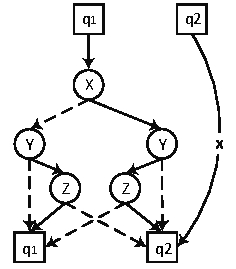
\includegraphics{fig/bdd-transition-function-encoding}
  \end{center}
  \caption{MTBDD coding transition function corresponding to the
  $\mathcal{A}_{\ref{word-automaton}}$ from example
  \ref{word-automaton}}\label{mtbdd}
 \end{figure}
 
\end{example}

\noindent\hrulefill

\chapter{The WS$k$S Logic}\label{wsks}
The abbreviation WS$k$S stands for \emph{weak second-order monadic logic of $k$
successors}. This means that it is a logic that allows quantification over set
variables (second-order), which can only represent \emph{finite} sets (weak) of
elements and \emph{not functions} (monadic), over a universe of discourse where
every element has $k$ successors, and can therefore express a tree structure
(for $k \geq 2$).
 
 \section{Syntax}
 A~WS$k$S \emph{term} is an empty constant $\epsilon$, a first-order variable
 symbol written in lower-case letters (e.g. \emph{x, y, z, \ldots}) or an unary
 symbol from $\{1,\ldots,k\}$ written in postfix notation.
 For example, $x1123$ or $\epsilon2111$ are terms, where the latter can be
 shortened to $2111$.

The \emph{atomic formulae} are defined as follows:
 \begin{enumerate}
  \item For terms $s$ and $t$, the equality $s = t$ is an atomic formula.
\item For terms $s$ and $t$, inequalities $s \leq t$ and $s \geq t$ are atomic
formulae.
\item For a term $t$ and a second-order variable $X$, the membership constraint
$t \in X$ is an atomic formula.
 \end{enumerate}

A WS$k$S \emph{formula} is then built out of atomic formulae using the
classical logical connectives $\wedge, \vee, \neg, \leftarrow, \rightarrow,
\leftrightarrow$ and quantifiers $\exists x, \forall x$ and $\exists X, \forall
X$ for quantification over first-order variables and second-order variables
respectively.

Syntax can be further restricted to only a subset of logical connectives and
atomic formulae without harm to the expressive power of the logic. This will be
further explained in Section \ref{restricted}. The set of \emph{free variables}
of a formula $\psi$ is defined as usual.
  
  \noindent\hrulefill
  \begin{example}
  The following example WS$k$S formula $\varphi$ denotes that there exists only
  one set that contains all elements from universe of discourse.
  \begin{equation}
   \varphi \overset{\mathit{def}}{=} \exists X: \forall p: p \in X \wedge
   \neg\exists Z:
   X = Z
  \end{equation}
   \hrulefill
  \end{example}\label{wsks-formula}
  
  \section{Semantics}
	
We will interpret terms as strings belonging to $\{1,\ldots,k\}^*$, $=$ as the
equality of strings, and $\leq$ as the prefix ordering. Second order variables
will be interpreted as \emph{finite} subsets of $\{1,\ldots,k\}^*$ with
$\in$ as the membership predicate.
	
Let $t_1,\ldots,t_n \in \{1,\ldots,k\}^*$ and $S_1,\ldots,S_n$ be finite subsets
of $\{1,\ldots,k\}^*$. Given a formula $\psi(x_1,\ldots,x_n,X_1,\ldots,X_m)$
with free variables $x_1,\ldots,x_n$, $X_n,\ldots,X_m$, the assignment $\delta =
\{ x_1 \mapsto t_1,\ldots, x_n \mapsto t_n, X_1 \mapsto S_1,\ldots, X_m \mapsto
S_m\}$ \emph{satisfies} $\psi$ written as $\delta \models \psi$ (or also
$t_1,\ldots, t_n, S_1,\ldots,S_m \models \psi$) if replacing the variables with
their corresponding values, the formula holds in the above model.
	
  \section{Restricting Syntax}\label{restricted}
	We are going to restrict the WS$k$S syntax to use only second-order variables.
	This can be done by considering every first-order variable as a singleton set
	and transforming every formula to an equivalent one which does not contain any
	first-order variables. We will consider only the following atomic formulae,
	where $X$ and $Y$ are second-order variables, and build formulae over them:
	\begin{itemize}
	 \item $X \subseteq Y$,
\item $\mathit{Sing}(X)$\,--\,holds true iff $X$ is a singleton set, \item $X
= Yi$\,--\,holds true iff $X$ and $Y$ are singleton sets $\{s\}$ and $\{t\}$
respectively and $s = ti$,
	 \item $X = \epsilon$.
	\end{itemize}
	
We can also further simplify the syntax of WS$k$S formulae by restricting
logical connectives used to build the formulae to only $\exists$, $\vee$ and
$\neg$.
	
	 This syntax will be called
the \emph{restricted syntax} and its satisfaction relation will be denoted as
$\models_2$.

  \noindent\hrulefill
  \begin{example}
  The following example WS$k$S formula $\phi$ is in restricted syntax and is
  equivalent to formula from Example \ref{wsks-formula}:
  \begin{equation}
   \phi \overset{\mathit{def}}{=} \exists X: \forall P: P \subseteq X \wedge
   \mathit{Sing}(P) \wedge \neg\exists Z: X = Z
  \end{equation}
   \hrulefill
  \end{example}\label{wsks-formula-restricted}
	
	\begin{prop}
There is a translation T from WS$k$S formulae to the restricted syntax such that
\begin{equation}
s_1,\ldots,s_n,S_1,\ldots,S_m \models
\psi(x_1,\ldots,x_n,X_1,\ldots,X_m)
\end{equation} if and only if \begin{equation}\{s_1\},\ldots,\{s_n\},S_1,\ldots,S_m \models_2
T(\psi)(X_{x_1},\ldots,X_{x_n}, X_1,\ldots,X_m)
\end{equation}.

 Conversely, there is a
translation $T'$ from the restricted syntax to WS$k$S such that \begin{equation}S_1,\ldots,S_m
\models T'(\psi)(X_1,\ldots,X_m)\end{equation} if and only if \begin{equation}S_1,\ldots,S_m \models_2
\psi(X_1,\ldots,X_m)\end{equation}.
	\end{prop}
	\begin{proof}
We will only present a short sketch of the proof for this proposition. For
further details see \cite{tata}.
	
We can suppose that formulae will be built only upon the atomic formulae $t \in
X$ and $s = t$ and so flatten the rest of the atomic formulae. Every first-order
variable $y$ will be mapped to a second-order variable $X_y$ as follows:
	
	 \begin{eqnarray}
	 T(y \in X) & \overset{\mathit{def}}{=} & X_y \subseteq X\\
	 T(y = xi) & \overset{\mathit{def}}{=} &  X_y = X_xi\\
	 T(x = \varepsilon) & \overset{\mathit{def}}{=} & X_x = \varepsilon\\
	 T(x = y) & \overset{\mathit{def}}{=} & X_x = X_y\\
	 T(\psi \vee \phi) & \overset{\mathit{def}}{=} & T(\psi) \vee T(\phi)\\
	 T(\neg\phi) & \overset{\mathit{def}}{=} & \neg T(\phi)\\
	 T(\exists X.\phi) & \overset{\mathit{def}}{=} & \exists X.T(\phi)\\
	 T(\exists y.\phi) & \overset{\mathit{def}}{=} & \exists X_y\ .\ Sing(X_y) \wedge T(\phi)
	 \end{eqnarray}
	Moreover, for each free variable $x$ we add a $Sing(X_x)$ formula. 
	
	The converse translation is $T'$ can be defined similarly as written
	in~\cite{tata}.
	\end{proof}
	
We will further restrict the syntax of WS$k$S. A~WS$k$S formula $\phi$ is in the
\emph{prenex normal form} (abbreviated as PNF) if and only if it is of the form
\begin{equation}
\phi = Q_1X_1Q_2X_2\ldots Q_nX_n\ .\ \psi(\mathds{X})
\end{equation} where 
$Q_i \in \{\exists,\forall\}$, $1 \leq i \leq n$, and $\psi$ is a quantifier-free formula
in the restricted syntax as defined above. We denote $Q_1X_1Q_2X_2\ldots Q_nX_n$
as the \emph{prefix} of $\phi$ and $\psi(\mathds{X})$ as the \emph{matrix} of
$\phi$.
	
A~WS$k$S formula $\rho$ is in the \emph{existentially-quantified prenex normal
form} (abbreviated as $\exists$PNF), if and only if \begin{equation}\rho =
\exists \mathcal{X}_{m+1}\neg\exists \mathcal{X}_m\ldots\neg\exists
\mathcal{X}_2\neg\exists \mathcal{X}_1.\psi(\mathds{X})
\end{equation} where
$\exists\mathcal{X}_i$, for $\mathcal{X}_i \subseteq \mathds{X}$, is a (possibly
empty) sequence $\exists X_a\ldots\exists X_b$ of consecutive existential
quantifications and $\psi$ is again a quantifier-free formula in the restricted
syntax over $\mathds{X}$.
	
  \noindent\hrulefill
  \begin{example}
  The following example WS$k$S formula $\psi$ is in existentially-quantified prenex normal
form and is equivalent to formula from Example \ref{wsks-formula}:
  \begin{equation}
   \psi \overset{\mathit{def}}{=} \exists X: \neg \exists P \exists Z: \neg P
   \subseteq X \vee X = Z \vee \neg\mathit{Sing}(P)
  \end{equation}
   \hrulefill
  \end{example}\label{wsks-formula-restricted}
	
	\begin{prop}
There is a translation from WS$k$S formulae in the restricted syntax to the
equivalent formulae in $\exists$PNF.
	\end{prop}
	
	\begin{proof}
Let us consider only $\wedge$, $\vee$ and $\neg$ is used in formulae as logical
operators. This can be achieved by applying rules $\psi \Leftrightarrow \phi
\mapsto (\neg \psi \vee \phi) \wedge (\psi \vee \neg \phi)$ and $\psi
\Rightarrow \phi \mapsto \neg \psi \vee \phi$, which preservers logical
equivalence.
	
Formula is first translated to the PNF, moving all quantifiers to the left
of formulae, renaming variables if needed. Quantifications with unbound
variables are removed. We are using the following transformations, where $Q \in
\{\exists, \forall\}$ and $\circ \in \{\vee, \wedge\}$:
	\begin{eqnarray}
	 \neg(\exists x \phi) & \equiv & \forall x\neg \phi\\
	 \neg(\forall x \phi) & \equiv & \exists x\neg \phi\\
	 Qx.\phi \circ \psi & \equiv & Qx(\phi \circ \psi)\label{one}\\
	 \phi \circ Qx.\psi & \equiv & Qx(\phi \circ \psi)\label{two}\\
	\end{eqnarray}
Note that there has to be no free occurrences of quantified variable $x$ in
$\psi$ and $\phi$ in formulae \ref{one} and \ref{two} respectively.
	
All universal quantifiers are transformed to existential quantifier
according to the equivalence $\forall x.\ \phi \equiv \neg\exists x.\ \neg\phi$.
Lastly all negations in the matrix are shifted to the atoms according to the
following laws:
	\begin{eqnarray}
	 \neg\neg\phi & \equiv & \phi\\
	 \neg(\phi\vee \psi) & \equiv & \neg \phi \wedge \neg \psi\\
	 \neg(\phi\wedge \psi) & \equiv & \neg \phi \vee \neg \psi 
	\end{eqnarray}
 The resulting formula is in the existentially-quantified prenex normal form. 
	\end{proof}
	
\section{Deciding WS$k$S}\label{classical}

A~decision procedure is an algorithm that given a formula $\phi$ returns VALID
if $\phi$ is valid, SAT if $\phi$ is invalid but satisfiable (additionally
yielding two assignments $\mathcal{M}_{true}$ and $\mathcal{M}_{false}$ such
that $\mathcal{M}_{\mathit{true}} \models \phi$ and
$\mathcal{M}_{\mathit{false}} \not\models \phi$) and UNSAT if $\phi$ is unsatisfiable.

Some properties of verified systems can be checked by being modeled by a set of
WS$k$S formulae and then deciding if the given formulae hold for all variable
assignments, therefore the checked system being valid, or either look for a
non-satisfying assignment which leads to violation of the specified properties..

The presented decision procedure for WS$k$S makes use of the close link between
WS$k$S formulae and automata, i.e.\ a given formula is transformed to
corresponding finite tree automata and its language is further examined. 

The contents of this section is based on the exposition over in \cite{tata}.

\begin{defz}
 A~set $L$ of tuples of finite sets of words is \emph{definable in WS$k$S} if
 there is a~formula $\psi$ of WS$k$S with free variables $X_1,\ldots,X_n$ such
 that \begin{equation}(S_1,\ldots,S_n) \in L \text{ if and only if }
 S_1,\ldots,S_n \models \psi.\end{equation}
\end{defz} Each tuple of finite sets of words $S_1,\ldots,S_n \subseteq
\{1,\ldots,k\}^*$ is then identified to a tree $(S_1,\ldots,S_n)^\sim$ over the
alphabet $\{0,1,\bot\}^n$ where any string containing 0 or 1 is $k$-ary and
$\bot^n$ is a constant symbol, such that
 \begin{equation}
  dom((S_1,\ldots,S_n)^\sim) \overset{\mathit{def}}{=} \{\epsilon\} \cup \left\{
  pi\ \Bigg|\ \exists p' \in \bigcup_{j = 1}^n S_j.p \leq p', 1 \leq i \leq
  k\right\}
 \end{equation}
The symbol at the position $p$: \begin{equation}(S_1,\ldots,S_n)^\sim(p) =
\alpha_1\ldots\alpha_n\end{equation} is defined as follows:
 \begin{itemize}
  \item $\alpha_i = 1 \text{ iff } p \in S_i$,
  \item $\alpha_i = 0 \text{ iff } p \notin S_i \wedge \exists p': p\cdot p' \in S_i$,
  \item $\alpha_i = \bot$ otherwise.
 \end{itemize}
 
\begin{lemma}
If a set of tuples of finite subsets of $\{1,\ldots,k\}^*$ is definable in
WS$k$S, then $\overset{\sim}{L} \overset{\mathit{def}}{=}
\{(S_1,\ldots,S_n)^\sim \mid (S_1,\ldots,S_n) \in L\}$ is in Rec.
\end{lemma}

\begin{proof}
 We have shown in Section \ref{restricted} that every formula in WS$k$S can be
 translated into an equivalent formula in the restricted syntax. We can now
 prove the lemma by induction on the structure of the formula $\psi$ which
 defines the language $L$.

Let us assume that all variables in $\psi$ are bound at most once in the formula
and also that there is a fixed total ordering $<$ on the variables.

If $\phi$ is a subformula of $\psi$ with free variables $Y_1 < \cdots < Y_n$, we
construct the automaton $\mathcal{A}_\phi$ over the alphabet $\{0,1,\bot\}^n$
such that $(S_1,\ldots,S_n) \models_2 \phi$ if and only if
$(S_1,\ldots,S_n)^\sim \in L(\mathcal{A}_\phi)$.
\end{proof}

In the following we limit ourselves to the case when $k = 2$; an extension to an
arbitrary $k$ is straightforward. As induction base, with for each atomic
subformula of $\psi$ we construct the automaton $\mathcal{A}_{\psi}$ according
to the following rules:
\begin{itemize}
 \item[-] The automaton $\mathcal{A}_{Sing(X)} = (\{q, q'\}, \{0, 1, \bot\},
 \delta, \{q'\}$) where $\delta$ is defined as follows:
\begin{eqnarray*}
  & \overset{\bot}{\longrightarrow} & q\\
 (q, q) & \overset{1}{\longrightarrow} & q'\\
 (q, q') & \overset{0}{\longrightarrow} & q'\\
 (q', q) & \overset{0}{\longrightarrow} & q'
\end{eqnarray*}
 \item[-] The automaton $\mathcal{A}_{X \subseteq Y} = (\{q\}, \{0, 1, \bot\}^2,
 \delta, \{q\}$), with $X < Y$, where $\delta$ is defined as follows:
\begin{eqnarray*}
  & \overset{\bot\bot}{\longrightarrow} & q\\
  (q, q) & \overset{00}{\longrightarrow} & q\\
  (q, q) & \overset{\bot 0}{\longrightarrow} & q\\
  (q, q) & \overset{01}{\longrightarrow} & q\\
  (q, q) & \overset{11}{\longrightarrow} & q\\
  (q, q) & \overset{\bot 1}{\longrightarrow} & q
\end{eqnarray*}
 \item[-] The automaton $\mathcal{A}_{X = Y1} = (\{q, q', q''\}, \{0, 1,
 \bot\}^2, \delta, \{q''\}$), where $\delta$ is defined as follows:
\begin{eqnarray*}
  & \overset{\bot\bot}{\longrightarrow} & q\\
  (q, q) & \overset{1\bot}{\longrightarrow} & q'\\
  (q, q'') & \overset{00}{\longrightarrow} & q''\\
  (q', q) & \overset{01}{\longrightarrow} & q''\\
  (q'', q) & \overset{00}{\longrightarrow} & q''
\end{eqnarray*}
Note that the automaton for $X = Y2$ is obtained similarly by changing $(q', q)
\overset{01}{\longrightarrow} q''$ to $(q, q') \overset{01}{\longrightarrow}
 q''$.
 \item[-] The automaton $\mathcal{A}_{X = \epsilon} = (\{q, q'\}, \{0, 1,
 \bot\}, \{q'\}, \delta$), where $\delta$ is defined as follows:
\begin{eqnarray*}
  & \overset{\bot}{\longrightarrow} & q\\
 (q, q) & \overset{1}{\longrightarrow}& q'
\end{eqnarray*}
\end{itemize}

Now as the induction step, we will consider only logical operations $\vee$,
$\wedge$, $\neg$ and $\exists$ (as defined in the restricted syntax):
\begin{itemize}
 \item[$\psi$]$ = \psi_1 \vee \psi_2$\,--\,let $\overline{X}_i$ be the set of
 free variables of $\psi_i$ respectively, and $\overline{X}_1 \cup
 \overline{X}_2 = \{Y_1,\ldots,Y_n\}$ with some ordering $Y_1 < \ldots < Y_n$.
 Then we successively apply the $i$-th cylindrification to the automaton of
 $\psi_1$ (resp. $\psi_2$) for the variables $Y_i$ which are not free in
 $\psi_1$ (resp. $\psi_2$), so the automata for $\psi_1$ and $\psi_2$ can
 recognize the solutions of $\psi_1$ and $\psi_2$, with free variables
 $\overline{X}_1 \cup \overline{X}_2$. Then the automaton $\mathcal{A}_\psi$ is
 obtained as the union of these automata.
 \item[$\psi$]$ = \psi_1 \wedge \psi_2$\,--\,is obtained similarly as automaton
 for connective $\vee$ by by using \emph{intersection} of automata.
 \item[$\psi$]$ = \neg\psi_1$\,--\,then $\mathcal{A}_\psi$ is the automaton
 accepting the complement of $L(\mathcal{A}_{\psi_1})$.
 \item[$\psi$]$ = \exists X.\psi_1$\,--\,assuming that $X$ corresponds to the
 $i$-th component, then $\mathcal{A}_\psi$ is the $i$-th projection of
 $\mathcal{A}_{\psi_1}$.
\end{itemize}

In implementation terms existential quantification is therefore equivalent to
operation of projection on automaton transition. This raises an issue with final
states of constructed automaton $\mathcal{A}$, since projection erases some of
the transition tracks of automaton and thus introduces non-determinism. Such automaton has to
be determinised yielding DTA $\mathcal{A}$'.

However automaton $\mathcal{A}'$ is not enough, since searched witness of some
model can be longer after operation of projection. Final states
$F_{\mathcal{A}'}$ has to be extended to include such states that can reach some
final states on strings of $\{\{0\}^k\}^*$. 

\begin{defz}
We define a \emph{right-quotient} of language $L$ with a language $L'$ as
\begin{equation}
 L / L' = \{w \mid \exists u \in L' : w\cdot u \in L\}
\end{equation}.
\end{defz}

Now we define a language $L^i$ as
\begin{equation}
 L^i = \{w \in \{\{0, 1\}^k\}^* \mid \text{the $j$-th track of word} \mathit{w}
 \text{is of the form $0^*$ for $j \neq i$}\}. \end{equation}
 
 So the language of automaton $\mathcal{A}'$ after projection $\gamma_i$ on
 $i$-th track of the transition is defined as
 \begin{equation}
  L(\mathcal{A}') = \gamma_i(L(\mathcal{A}) / L^i).
 \end{equation}
 
 In \textsc{MONA} \cite{mona} this is done in $\mathcal{O}(n)$ time by using
 breath-first search by backwards exploration of the automaton from final
 states followed by subset construction of determinised automaton yielding only
 reachable states.

\begin{prop}
 Since there is a \emph{one-to-one} correspondence between models of $\phi$ and
 trees accepted by $\mathcal{A}_\phi$, $\phi$ is satisfiable iff
 $L(\mathcal{A}_\phi)$ is non-empty and valid iff $L(\mathcal{A}_\phi)$  is
 universal.
\end{prop}

  \noindent\hrulefill
  \begin{example}
  Consider following WS$k$S formula:
  \begin{equation}
  \rho \overset{\mathit{def}}{=} \exists P:
 Sing(P) \wedge P \not\subseteq X
  \end{equation}
  Deciding validity of $\rho$ consists of constructing automaton
  $\mathcal{A}_\rho$ corresponding to the formula $\rho$ and then afterward
  check the language $L(\mathcal{A}_\rho)$ for universality, i.e. if any
  non-accepting state is reachable. As depicted in Figure \ref{automata} we
  first construct automata $\mathcal{A}_{\mathit{Sing}(P)}$ and
  $\mathcal{A}_{P \not\subseteq X}$ for subformulae $\mathit{Sing}(P)$ and $P
  \not\subseteq X$ respectively. Then we construct product automaton of those
  subformulae yielding automaton $\mathcal{A}_{\mathit{Sing}(P) \wedge } P
  \not\subseteq X$. Finally we make a projection of automaton by erasing track
  corresponding to the quantified variable $P$ and obtain the resulting
  automaton $\mathcal{A}_\rho$.

  \end{example}\label{wsks-formula-restricted}
 
 \begin{figure}[h!]
 \begin{center}
  \scalebox{0.55}{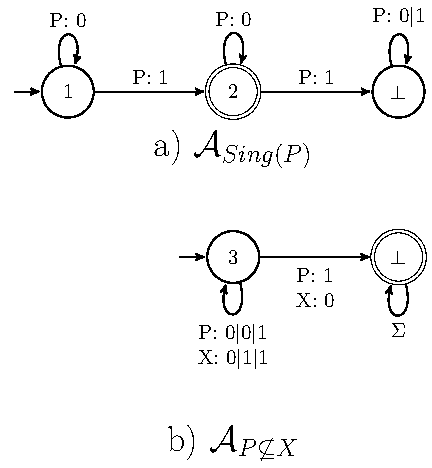
\includegraphics{fig/formula-singleton-and-subset.pdf}}
  \scalebox{0.55}{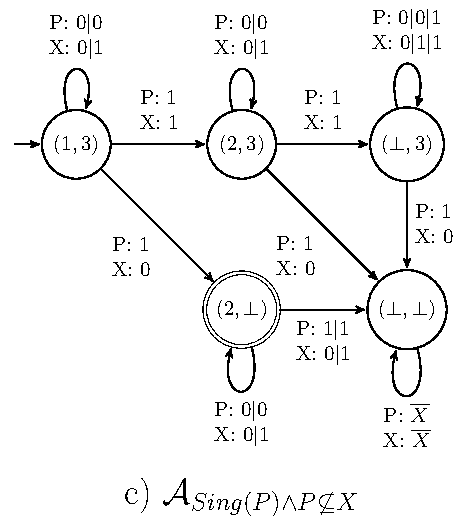
\includegraphics{fig/formula-automaton-product.pdf}}
  \scalebox{0.55}{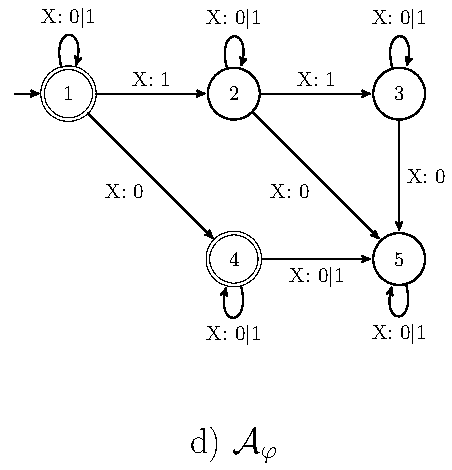
\includegraphics{fig/formula-automaton.pdf}}
 \end{center}
 \caption{Finite automata corresponding to the subformulae of the formula
 $\rho \overset{\mathit{def}}{=} \exists P:
 Sing(P) \wedge P \not\subseteq X$}\label{automata}
\end{figure}
   \noindent\hrulefill

The computational complexity of WS$k$S is in NONELEMENTARY class, so given
a Turing machine $\mathcal{M}$ deciding a satisfiability of WS$k$S formulae, for
any $u \geq 0$, there are infinitely many $n$ for which a computation of
$\mathcal{M}$ for some sentence of length $n$ requires at least
$$\underbrace{2^{2^{\iddots^{2^n}}}}_u$$ steps.
	
\chapter{\textsc{MONA}}\label{monachap}

 \textsc{MONA} \cite{mona} is one of the early implementations of decision
 procedures for the WS$k$S logic, namely for $k = 1$ and $k = 2$ (note that it
 can be shown, that arbitrary $k$ can be transformed to formula in WS2S). WS1S
 can be used for description of linear structures like linked lists or chains,
 while WS2S is mainly used for binary tree structures like binary tree or binary
 heap. For many years it is still the best and fastest approach for decision of
 the formulae with usage of deterministic automata. It is an implementation of
 the decision procedure from Chapter \ref{classical} with a few tweaks that we
 describe in this chapter

\textsc{MONA} has been developed since 1994. Through all these years numerous
approaches were tried out and thus number of fine optimizations were discovered.
In this chapter we review some of the designed and implementation tricks that
stand behind its success. Even though, the overall complexity is still
non-elementary for the worst-cases.

\section{Main issue of using deterministic tree automata}

Considering WS$k$S formula with a fixed number of quantifier alternations $N$,
the decision method outlined in the previous section works in time which is a
tower of exponentials with height being $O(N)$.

This is mainly because every time we encounter a sequence of quantifiers, we
have to do a projection, which yields a non-deterministic automaton, even if the
input automaton was deterministic. Now when we encounter a negation of a
formula, we have to use determinization before doing a complement of automaton,
which requires in general exponential time and exponential space w.r.t states of
automata.

So every time non-determinism is introduced to automaton it is determinised and
the information about the original states is forgotten. So \textsc{MONA}
approach has issues with extensive us of automaton complementation and since there
is no known tree automaton complementation technique better than bottom-up
determinization of automaton with complementation of the set of final states,
\textsc{MONA} had to come up with heavy optimizations and heuristic to achieve
good results.

 \section{Used optimizations}\label{monasecrets}
\subsection{Using BDDs for automata representation}\label{monabdd}
BDDs were introduced to solve the problems of large input alphabets, which also
allowed numerous specialized algorithms to be used.

BDDs were described in Section \ref{bdd}, and are useful for its compactness,
canonicity and efficient manipulation. \textsc{MONA} uses shared MTBDDs with
roots and leaves representing the states. The use of BDDs for representation  of
transition relation proved to have the highest effect on formulae that could not
be decided in fixed limit of a time that was set up during benchmarks.

\subsection{Caching}
The implementation of the BDDs, as stated in Section \ref{monabdd}, is optimized
to minimize the number of cache misses that occur, since it was discovered that
cache misses dominate the running time for both the unary and binary BDD apply
operations.

Nodes are thus stored directly under the hash address to minimize the cache
misses, as opposed to the traditional approach that stores nodes separately from
the hash table containing pointers to them, which roughly doubles the time to
process a node.

\subsection{Eager minimization}
Whenever MONA performs the product or projection operation during the
translation from formula to an automaton, the Myhill-Nerode minimization takes
place, since it is preferable to operate with as small automata as possible.
However this approach was shown to be excessive, since minimization procedure
often exceeds half of the total running time.

Alternatives were introduced\,--\,using one final minimization, minimizing only
after projection or minimizing only after product, which had different effects
and were dependent on concrete benchmarks.

\subsection{Guided tree automata}

The set of states is partitioned in order to split a large tree automata into
the smaller ones to address expensive computations caused by three-dimensional
transition tables. This however requires for user to specify the \emph{guide}
which is a top-down deterministic tree automaton that assigns state spaces to
the nodes of a tree.

\subsection{Directed Acyclic Graph representation}\label{dag}

The frontend of the MONA tool is parsing the input files with specification of
WS$k$S formulae. This file is converted to the inner representation of
automata-theoretic operations, that are further translated to resulting
automaton.

There are however many common subformulae with similar structure, especially if
we talk about \emph{signature equivalence}, which holds for two formulae $\phi$
and $\psi$ if there is an order-preserving renaming of the variables in formulae
such that the representations of $\phi$ and $\psi$ become identical.

It holds for BDD representation that automata for signature-equivalent trees are
isomorphic in the sense that only node labels differ, which means this
representations can be reused simply by renaming the variables nodes. Thus MONA
represents input formulae in the form of \emph{directed acyclic graph} and not a
tree.

\subsection{Three-valued logic and automata}
Since formulae are translated to the restricted syntax that uses only
second-order variables, first-order variables are encoded as singletons. This
however raises the issue of \emph{restrictions}, i.e. the formula $\phi$ holds
only when some external associated restrictions hold. Since restriction is also
a formula, the main issue is that $\phi$ is now undefined outside the
restriction. Note that for a first-order variable, the restriction is that it is
a singleton set.

The nature of these problems are solved by using a three-valued logic. So for a
restricted subformula $\phi$ we associate a restriction $\phi_R$. And if for
some valuation $\phi_R$ does not hold, then the formulae containing $\phi$ are
assigned the third value \emph{dont-care}.

A~special operation converts the rejecting states to dont-cares for the
restriction formulae and other automaton operations are modified so these
nonacceptance of restrictions are propagated properly.

\subsection{Formula reductions}
Various optimizations of formulae takes place in the DAG specified in Section
\ref{dag} before the final translation to automata. Reductions are based on
syntactic analysis that tries to identify valid subformulae and equivalences
among them.

MONA performs three kinds of reductions:
\begin{enumerate}
 \item Simple equality and Boolean reductions that can be described by simple
 rewrite rules like $\phi \wedge \phi \Leftrightarrow \phi$, etc. These rewrite
 steps guarantee a reduction of complexity, but will not cause significant
 improvements in the running time, since they rarely apply in realistic
 situations. However they are cheap and may yield small improvements.

\item Special quantifier reductions. The basic idea is to apply a rewrite step
which removes quantifiers, where they are not useful, as following: 
\begin{equation}\exists X
. \phi \Leftrightarrow \phi[T/X]\end{equation} provided that $\phi \Rightarrow
X = T$ is valid and $T$ is some term satisfying $freevar(T) \subseteq freevar(\phi)$,
where $freevar$ denotes the set of free variables of subformula. This is further
restricted to different rewrite rule: \begin{equation} \exists X_i . \phi \Leftrightarrow
\phi[X_j/X_i]\end{equation} provided that $\phi \equiv \ldots \wedge X_i = X_j \wedge
\ldots$ and $X_j$ is some variable other than $X_i$. This, however, is not
guaranteed to yield better results.

\item Special conjuction reductions. There are two sources of reductions. The
first is formula flattening. The other is  the formula restriction mentioned
above.
\end{enumerate}

 \chapter{Deciding WS$k$S with Non-deterministic Automata}\label{our}

The \textsc{MONA} tool implementation of the decision procedure for WS$k$S from
Section \ref{classical} uses deterministic bottom-up tree automata (as described
in Chapter \ref{monachap}) and so every time non-determinism might be
introduced, such as through union and projection corresponding to disjunction
and existential quantification respectively, the automaton is determinised using the
subset construction and the information about the original states is forgotten.

While this approach makes automaton complementation ease (since deterministic
automata require only swapping final with non-final states), the extensive
determinisation is still a serious drawback. The \textsc{MONA} tool is
thus heavily optimized for the use of deterministic finite (tree)
automata, as we introduced in Section \ref{monasecrets}. However, a decision
procedure that uses non-deterministic automata needs to deal with the issue of
complementation, for which there is currently no known algorithm that avoids
determinisation and the respective state explosion.

In practice, the representation of all models of $\phi$ is not always necessary
and any model or an invalid assignment to free variables suffices, therefore
constructing the automaton $\mathcal{A}_{\phi}$ representing all models of
$\phi$ can be avoided.

Current trends in formal verification and theory of automata tend to use
non-deter\-ministic automata instead of deterministic ones. This is due to the
fact that there exist optimized libraries for their use, like VATA
\cite{vata}, and recently new algorithms that are efficient in practice
were developed even for time complex operations like language inclusion or
universality testing, which are PSPACE-complete for finite word automata and
EXPTIME-complete for tree automata.

Here we propose to use an algorithm based on the principle of antichains
\cite{tacas}, defined in the following sections, and search for an accepting
or non-accepting state \emph{on-the-fly} without constructing the automaton
corresponding to the given formula in the first place.

\section{Antichain-based universality testing of NFAs}

We will give a brief introduction to universality testing for non-deterministic
finite word automata by an algorithm that uses a combination
of the simulation-based and the antichain-based approaches \cite{tacas}.

\begin{defz}
A~\emph{simulation} on a finite automaton $\mathcal{A} = (Q, \Sigma, \delta, I,
F)$ is a relation $\preceq \subseteq Q \times Q$ such that $p \preceq r$ implies
the following two conditions (i) $p \in F \Rightarrow r \in F$ and (ii) for
every transition $p \overset{a}{\longrightarrow} p'$, there exists a transition $r
\overset{a}{\longrightarrow} r'$ such that $p' \preceq r'$.
\end{defz}

Further we call a set of states in $\mathcal{A}$, i.e. a subset of $Q$, a
\emph{macro-state} and we use $A^{\subseteq}$ to denote a set of relations over
the states of $\mathcal{A}$ that imply language inclusion, that is for all
$\leqq \in A^{\subseteq}$ $p \leqq r \Rightarrow L(p) \subseteq L(r)$.

\begin{lemma}
Given a simulation $\preceq \in A^{\subseteq}$ on a NFA $\mathcal{A}$, $p
\preceq r \Rightarrow L_\mathcal{A}(p) \subseteq L_\mathcal{A}(r)$.
\end{lemma}

\begin{proof}
A proof can be found in \cite{tacas}.
\end{proof}

The universality problem for a NFA $\mathcal{A} = (Q, \Sigma, \delta, I, F)$ is
to decide whether $L(\mathcal{A}) = \Sigma^*$. The problem is PSPACE-complete.

The naive algorithm performs determinization using a subset construction to
obtain a~deterministic automaton $\mathcal{A}_D$, then complements it to obtain
$\overline{\mathcal{A}_D}$ and finally checks that there is no reachable
accepting state in $\overline{\mathcal{A}_D}$ (in case there is, the language
is not universal).

The algorithm proposed in \cite{tacas} runs the subset construction procedure
on-the-fly, avoiding explicit construction of $\overline{\mathcal{A}_D}$, and
checks if any accepting macro-state is reachable. This procedure is
further augmented with two optimizations. We define the post-image of a~state as
$Post(p) = \{p'\in Q \mid \exists a \in \Sigma: (p, a, p') \in \delta\}$.

The first optimization is based on the following lemma.

\begin{lemma}\label{lemma2}
 Let $P, R$ be two macro-states of a NFA $\mathcal{A}$, and $\preceq$ be a
 relation from $\mathcal{A}^\subseteq$. Then, $P \preceq^{\forall\exists} R$
 implies $L_\mathcal{A}(P) \subseteq L_\mathcal{A}(R)$, where $P
 \preceq^{\forall\exists} R$ stands for $\forall p \in P. \exists r\in R : p
 \preceq r$.
\end{lemma}

The relation $\preceq$ can be any relation on the states of $\mathcal{A}$ that
implies language inclusion, e.g. the maximum simulation or the identity
relation. The other optimization is based on the observation that
$L_\mathcal{A}(P) = L_\mathcal{A}(P - \{p_1\})$ if there is some $p_2 \in P \setminus \{p_1\}$ such
that $p_1 \preceq p_2$, which is a simple consequence of Lemma \ref{lemma2}.

\begin{algorithm}[ht!]
		\SetKwFor{For}{foreach}{do}{}
		\SetKwRepeat{Repeat}{repeat}{until}
		\KwIn{A macro-state $I$ of automaton $\mathcal{A}$, a simulation relation
		$\leqq \subseteq A^{\subseteq}$ on states of
		$\mathcal{A}$, a successor function $\delta$ and a predicate
		\texttt{IsFinal(F)} that decides whether a macro-state $F$ is final}
		\KwOut{\textsc{TRUE} iff there exists a reachable final state in
		$\mathcal{A}$,
		\textsc{FALSE} otherwise}
		\BlankLine
				\SetKwProg{myproc}{Function}{}{}
		\BlankLine
  \myproc{\upshape \texttt{IsFinalReachable}(\textbf{state} I, level i,
  \textbf{post function} $\delta$, \textbf{pred} \texttt{IsAccepting})}{
    \nl\uIf{\upshape \texttt{IsFinal}(I)}{
    	\nl\Return \textsc{TRUE}\;}
		\nl $Processed := \emptyset$\;
		\nl $Next := \{I\}$\;
		\nl\While{$Next \neq \emptyset$}{
		  \nl Pick and remove a macro-state $R$ from $Next$ and move it to
		  $Processed$\;
			 \nl \uIf{\upshape \texttt{IsFinal}(R)}{\nl \Return \textsc{TRUE}\;}
			\nl \For{$P \in \delta(R)$}{
			 \nl \uIf{$\neg\exists S~\in Processed \cup Next$ s.t. $P \leqq S$}{
			  \nl Remove all $S$ from $Processed \cup Next$ s.t. $S \leqq P$\;
				\nl Add $P$ to $Next$\;
			 }
			}
		}
		\nl \Return \textsc{FALSE}\;
		}
		\caption{Checking reachability of a
		final state using optimized algorithm\cite{tacas}}\label{universality}
	\end{algorithm}
	
The algorithm \ref{universality} works as follows. While there are macro-states
to be processed, and no accepting macro-state has been found, one of the macro-states from $Next$
is chosen and moved to the $Processed$ set. All successors of the macro-state are
generated, minimized and moved to $Next$ unless there is already some
$\preceq$-smaller macro-state in $Next$ or in $Processed$. If a
new macro-state is added to $Next$, then all the
$\preceq$-bigger states are pruned out of both $Next$ and
$Processed$.

Testing the universality of an automaton $\mathcal{A}$ is equivalent to
searching for an accepting state in automaton $\mathcal{A}'$ obtained by
determinization and complementation of final states.
	
\begin{lemma}\label{search-is-correct}
 Given the automaton $\mathcal{A}$, function \texttt{CheckForReachableState()}
 \ref{universality} returns \textsc{TRUE} iff there is a reachable accepting
 state in $\mathcal{A}$.
\end{lemma}
\begin{proof}
 A proof can be found in \cite{raskin}.
\end{proof}

\begin{lemma}\label{simulation-in-ca}
Relation $\subseteq^{-1}$ is a simulation on the complemented automaton
$\mathcal{A}'$.
\end{lemma}
\begin{proof}
 Proof can be found in \cite{raskin}
\end{proof}

\begin{lemma}
The language of automaton $\mathcal{A}$ is universal if the Algorithm
\ref{universal} returns \textsc{TRUE}
\end{lemma}

\noindent\hrulefill
\begin{example}
Consider testing validity of a formula $\varphi$ from Example
\ref{wsks-formula}.
Given automaton $\mathcal{A}_\varphi$ corresponding to the formula $\varphi$
(see Section \ref{classical}), testing validity of $\varphi$ is
equivalent to testing universality of the language $L(\mathcal{A}_\varphi)$.

When using the textbook approach for testing universality (by using the subset
construction and complementation), 7 states are generated as depicted in Figure
\ref{compare} If we use the antichain-based approach, then macro-states $\{1,
2\}$ and $\{1, 4\}$ are simulated by the initial state $\{1\}$ so we can
discard these states.
Since we have not reached an accepting state, we can conclude that the language
of the automaton $\mathcal{A}_\varphi$ is not universal and $\varphi$ is thus
invalid.
\end{example}

\noindent\hrulefill

\begin{figure}
 \begin{center}
  \scalebox{0.5}{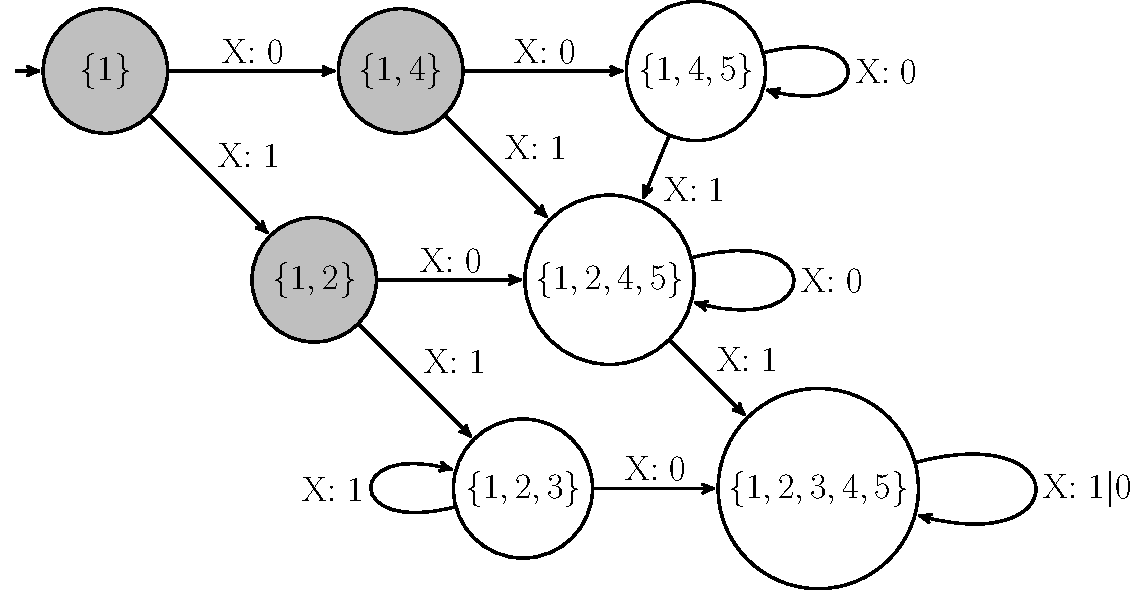
\includegraphics{fig/antichain-meets-projection.pdf}}
 \end{center}
 \caption{Comparison of the antichain-based (grey nodes) and the classical (all
 nodes) approach to universality checking of the automaton $\mathcal{A}_\psi$
 corresponding to the formula $\psi \overset{\mathit{def}}{=} \neg\exists P:
 Sing(P) \wedge\neg P \subseteq X$}\label{compare}
\end{figure}

\section{Deciding WS1S with NFAs}

Given formula $\phi$, construction of the automaton $\mathcal{A}_\phi$
representing all models of $\phi$ is not always necessary and in many
applications any model or an invalid assignment suffices.
Therefore we can exploit the antichain-based techniques defined in previous
section and search for an accepting or non-accepting state \emph{on-the-fly}
while pruning the search space.

First, the formula $\phi$ is transformed to a logically equivalent formula
$\varphi$ in the existential prenex form (see Section \ref{restricted}):
\begin{equation*}
 \varphi \overset{\mathit{def}}{=}
 \exists\mathcal{X}_{m+1}\neg\mathcal{X}_m\neg\ldots\neg\exists\mathcal{X}_2\neg\exists\mathcal{X}_1
 :
 \pi.
\end{equation*}

Supposing there are $m$	negations in the prefix of the formula $\varphi$, we
create a hierarchical family of WS$k$S formulae $\Phi = \{\varphi_0,\ldots,\varphi_m\}$
where
\begin{equation}
  \varphi_0 \overset{\mathit{def}}{=} \pi
\end{equation}
and for all $0 \leq i \leq m-1$
\begin{equation}
 \varphi_{i+1} \overset{\mathit{def}}{=} \neg\exists\mathcal{X}_{i+1}.
 \varphi_i.
\end{equation}
The relation between this family of formulae $\Phi$ and the formula $\varphi$ is
depicted as follows:
\begin{equation}
\begin{aligned}
\varphi = \exists \mathcal{X}_{m+1}\,
\underset{\varphi_m}{\underbrace{
  \neg\,\exists \mathcal{X}_m\,
  \neg
  \underset{\hspace{-3mm}\iddots}{
    \dots 
    \underset{\varphi_2}{\underbrace{
      \neg \,\exists \mathcal{X}_2\,
      \underset{\varphi_1}{\underbrace{
        \neg \,\exists \mathcal{X}_1\,.\,
        \underset{\varphi_0}{\underbrace{
          \pi
        }}
      }}
    }}
  }
}}
\end{aligned}
\end{equation}

We will use $\Gamma(G)$ to denote the alphabet defined as the
set of functions $\Theta(G) = \{f : G \rightarrow \{0, 1, \bot\}\}$, with the
special case for $G = \emptyset$ defined as $\Gamma(\emptyset) = \{\#\}$. Elements of this set can
be viewed as strings of a fixed length $|G|$ over the alphabet $\{0, 1, \bot\}$
where each position in the strings is associated with exactly one element of G.

Now, given the symbol $f \in \Gamma(G)$ and a set $H \subseteq G$ the
\emph{projection} of $f$ over the set $H$, written as $\omega_H(f)$, can be
defined as the restriction of the function $f$ over the set $G\setminus H$, i.e.
$\omega_H(f) = f|_{G\setminus H}$. This can be further extended to sets of symbols. Given a
set $E \subseteq \Gamma(G)$, we define the projection over a set $H \subseteq
G$, written $\omega_H(E)$, as $\omega_H(E) = \{\omega_H(f) \mid f \in E\}$.

For a language $L \subseteq \Gamma(G)^*$, the projection of $L$ over $H$,
written as $\omega_H(L)$, is defined as $\omega_H(L) = \{\omega_H(f) \mid f \in
L\}$. Note that $\omega_H(L) \subseteq \Gamma(G\setminus H)^*$.

\begin{lemma} Given the alphabet $\Gamma(G)$, $H \subseteq G$ and $X, Y
\subseteq \Gamma(G)^*$ it holds that
\begin{equation}
 X \subseteq Y \Longrightarrow \omega_H(X) \subseteq \omega_H(Y).
\end{equation}
\end{lemma}
\begin{proof}
For each symbol $z \in \omega_H(X)$ there must exist some $x \in X$ such that
$z = \omega_H(x)$. Since $X \subseteq Y$ it must also hold that $x \in Y$, and
hence $\omega_H(x) \in \omega_H(Y)$. Therefore $\omega_H(X) \subseteq
\omega_H(Y)$.
\end{proof}

As we described in Section \ref{wsks}, there is an issue with the encoding of
all models and using the projection operation on automata. After the projection the
automaton corresponding to a formula does not accept some of the valid models
of formula, as described by Example \ref{models}. \textsc{MONA} (see Section
\ref{classical}) solves this by adjusting the final states of the automaton by
using the bread-first search algorithm in linear time after every projection of
automaton.

\noindent\hrulefill
\begin{example}
 Consider the formula $P \not\subseteq X$ and its corresponding automaton
 $\mathcal{A}_{P \not\subseteq X}$ depicted in Figure \ref{projection} with one
 final state.
 After projection over the track corresponding to the variable $P$ we get the
 automaton $\mathcal{A}_{\exists P: P \not\subseteq X}b$ in Figure
 \ref{projection}b.
 
 After the projection the automaton does not accept e.g. the word $111 \notin
 L(\mathcal{A}_{\exists P: P \not\subseteq X})$ even though the set $X = \{1, 2,
 3\} \models \exists P: P \not\subseteq X$. However, it does accept another
 encoding of this set $1110 \in L(\mathcal{A}_{\exists P: P \not\subseteq X})$,
 which is not a correct encoding according to the rules set in Chapter
 \ref{wsks}. Hence we must adjust the final states.
 
 \begin{figure}[h!]
  \begin{center}
   \scalebox{0.75}{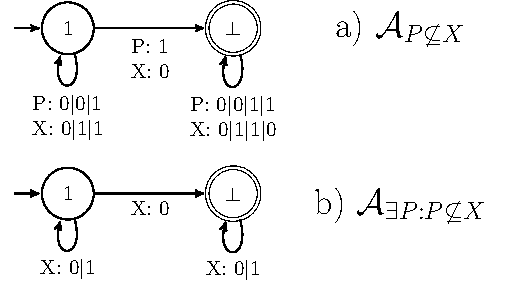
\includegraphics{fig/projection-problem}}
  \end{center}
  \caption{The issue with final states after projection is that
  the language of the resulting automaton restricts encodings
  of some valid models afterwards.}\label{projection}
 \end{figure}\label{models}
\end{example}
\noindent\hrulefill

However, this approach needs a fully constructed automaton, so this cannot be
used in an on-the-fly algorithm. Instead, we can either precompute the set of
inspired by backwards universality testing \cite{backwards-universality} or use
a lazy approach that will determine whether a state is final only when this
information is needed.

Note that in the following we will use the symbol $\overline{0}$ as the
substitute for symbol $0^k$, for some known $k$.

\begin{defz}
For a set of states $Q$ of automaton $\mathcal{A} = (Q, \Sigma, \delta, I, F)$
we define the \emph{set of predecessors through zero tracks} as the set $\mathit{PRE}_0(Q)$ of states such that
\begin{equation}
 \mathit{PRE}_0(Q) = \{r \in Q \mid \exists q \in Q: r
 \overset{\overline{0}}{\longrightarrow} q \in \delta\}.
\end{equation}
We denote the reflexive transitive closure of $PRE_0(Q)$ as $PRE_0^*(Q)$. Note
that we can define the $POST_0(Q)$ function similarly to $PRE_0$.
\end{defz}

\begin{defz}
 Given the automaton $\mathcal{A} = (Q, \Sigma, \delta, I, F)$ we define the
 \emph{projection} $\omega_\mathcal{X}$ over the set of variables $\mathcal{X}$
 of $\mathcal{A}$ as the automaton $\omega_\mathcal{X}(\mathcal{A}) = (Q,
 \omega_{\mathcal{X}}(\Sigma), \omega_{\mathcal{X}}(\delta), I, PRE_0^*(F))$
 where
 \begin{equation}
  \omega_{\mathcal{X}}(\delta) = \left\{ p \overset{\omega(a)}{\longrightarrow}
  r \mid p \overset{a}{\rightarrow} r \in \delta, a \in \Sigma\right\}.
 \end{equation}
 Note that after the operation of projection we have to adjust the final states
 according to the $PRE_0$ relation.
\end{defz}

\begin{defz}
 Given the automaton $\mathcal{A} = (Q, \Sigma, \delta, I, F)$ we define the
 \emph{complementation} $\gamma$ of $\mathcal{A}$ as the automaton
 $\gamma(\mathcal{A}) = (2^Q, \Sigma, \delta_\gamma, \{I\}, \{S \subseteq Q\
 |\ S \cap F = \emptyset\})$ where
 \begin{equation}
  \delta_\gamma = \{R \overset{a}{\rightarrow} S \mid S = \{s \in Q \mid \exists
  r \in R: r \overset{a}{\rightarrow} s\}\}
 \end{equation}
 Note that this operation $\gamma$ corresponds to the determinisation of the
 input automaton using the subset construction followed by swapping final and
 non-final states of the determinised automaton.
\end{defz}

We will first outline our new approach to deciding WS$k$S on WS$1$S formulae and
later generalize it to arbitrary $k$, which is quite straightforward.

Given a WS$1$S formula $\varphi$ in the $\exists$PNF form, the automaton for
the matrix $\pi$ of the formula, $\mathcal{A}_\pi$, can be constructed out of
automata corresponding to the atomic formulae and their complements by using operations of union and
intersection only. Further, we could construct $\mathcal{A}_\varphi$ from
the automaton $\mathcal{A}_\pi$ by successive applications of complementation
$\gamma$ and projection $\omega$ according to the prefix of $\varphi$, as these
operations were defined in Section \ref{preli}. But we take a different path.

% \begin{defz}
%  We define the \emph{downward closure} of a set $S$ as set $\downarrow S$ such
%  that
%  \begin{equation}
%   \downarrow S \overset{\mathit{def}}{=} \{p\in Q \mid \exists q \in S: p
%   \subseteq q\}
%  \end{equation}
% \end{defz}
% 
% \begin{defz}
%  Similarly we define the \emph{upward closure} of a set $S$ as set $\uparrow S$
%  such that
%  \begin{equation}
%  \uparrow S \overset{\mathit{def}}{=} \{p\in Q \mid \exists q \in S: q \subseteq
%  p\}
%  \end{equation}
% \end{defz}

% \begin{defz}
%  We define the \emph{preset through zero tracks} as a set of states such that
%  \begin{equation}
%  PRE_0(Q) = \{r \mid \exists q \in Q: r \overset{(0)^k}{\longrightarrow}
%  q\}.\footnote{Note that $(0)^k$ does stand for zero track of width $k$ not
%  length.}
%  \end{equation}
%  We denote the transition closure of $PRE_0(Q)$ as $PRE_0^*(Q)$. Note that we
%  can define the $POST_0(Q)$ relation simiralry to the $PRE_0$ relation.
% \end{defz}

Analogously to the family of formulae $\Phi$, we can define
the family of automata $\mathbb{A} = \{\mathcal{A}_0,\ldots,\mathcal{A}_m\}$ as follows:
 \begin{eqnarray}
  \mathcal{A}_0 & = & \mathcal{A}_\pi\\
  \mathcal{A}_{i+1} & = & \gamma(\omega_{\mathcal{X}_{i+1}}(\mathcal{A}_i)).
 \end{eqnarray}
 
 Note that the automaton $\mathcal{A}_i$ then corresponds to the following
formula:
 \begin{equation} \mathcal{A}_i =
 \exists\mathcal{X}_i\ldots\neg\exists\mathcal{X}_1.
 \pi(\mathbb{X}).
 \end{equation}
 
 We use the notation $\mathcal{A}_i = (Q_i, \Sigma_i, \delta_i, I_i, F_i)$ to
 address a particular automaton and its components.
There is a further connection between the hierarchical family of formulae $\Phi$
and the hierarchical family of automata $\mathbb{A}$ as described by the
following lemma.
 \begin{lemma} For all $0 \leq i \leq m$, the language of
$\mathcal{A}_i$ is
\begin{enumerate}
  \item \emph{universal} iff $\varphi_i$ is \emph{valid},
  \item \emph{non-empty} iff $\varphi_i$ is \emph{satisfiable},
  \item \emph{non-universal} iff $\varphi_i$ is \emph{invalid}, and
  \item \emph{empty} iff $\varphi_i$ is \emph{unsatisfiable}.
\end{enumerate}
\end{lemma}\label{uni-valid}

\begin{proof}
Proof of this Lemma can be found in \cite{tata}.
%  This can be proved by induction on $i$. With base case $i = 0$ holding due to a
%  proposition \ref{prop}. We can further prove this lema for case $i = n + 1$
%  supposing it holds for some $n$, i.e. the language of $\mathcal{A}_n$ is
%  \begin{enumerate}
%    \item universal iff $\varphi_n$ is valid,
%    \item non-empty iff $\varphi_n$ is satisfiable,
%    \item non-universal iff $\varphi_n$ is invalid, and
%    \item empty iff $\varphi_n$ is unsatisfiable.
%  \end{enumerate}
%  
%  We define the formula $\varphi_{n+1}$ as 
%  \begin{equation}
%  \varphi_{n+1} \overset{\mathit{def}}{=} \neg\exists\mathcal{X}_{n+1}.
%  \varphi_n.
%  \end{equation}
%  
%  Now we will consult each of the cases of the validity, or satisfiablity, of
%  given formula $\varphi_n$:
%  \begin{enumerate}
%    \item Suppose that $\varphi_n$ is valid. Then after the projection over set
%    of variables $\mathcal{X}_{n+1}$ the formula is still valid and the negation
%    of the formula $\varphi_{n+1} = \neg\exists\mathcal{X}_{n+1}.\varphi_n$ is
%    thus unsatisfiable. By the induction hypothesis it holds, that the language
%    $L(\mathcal{A}_n)$ is universal. After projection the language
%    $\omega_{\mathcal{X}_{n+1}}(L(\mathcal{A}))$ is also universal and the
%    negation thus makes the language $L(\mathcal{A}_{n+1})$ empty.
%    \item Suppose that $\varphi_n$ is satisfiable. Then after projection formula
%    $\exists\mathcal{X}_{n+1}. \varphi_n$ is also satisfiable (since, the
%    projection yields bigger or equivalent language) and the negation of the
%    formula $\varphi_{n+1} = \neg\exists\mathcal{X}_{n+1}.\varphi$ is thus
%    invalid. From induction hypotesis it holds that the language
%    $L(\mathcal{A}_n)$ is non-empty. After the projection the language remains
%    non-empty and so the negation of the formula yields non-universal language
%    $L(\mathcal{A}_{n+1})$.
%    \item Suppose that $\varphi_n$ is unsatisfiable. Then after projection
%    formula $\exists\mathcal{X}_{n+1}$ is still unsatisfiable, which means that
%    the negation of the formula $\neg\exists\mathcal{X}_{n+1}$ is valid. By
%    induction hypothesis the language $L(\mathcal{A}_n)$ is empty. The projection
%    of the language $\omega_{\mathcal{X}_{n+1}}(L(\mathcal{A}_n))$ is still empty
%    and so the negation of the formula yields univesal language.
%    \item Suppose that $\varphi_n$ is invalid. Then after projection formula
%    $\exists\mathcal{X}_{n+1}$ can either be still invalid or can become valid,
%    after the augmentation of the final states. Thus we have to distinguish two
%    cases:
%    \begin{enumerate}
%      \item Let us assume thet formula $\exists\mathcal{X}_{n+1}\varphi_n$ is
%      invalid.
%      Then after negation formula $\neg\exists\mathcal{X}_{n+1}\varphi_n$ is
%      satisfiable. By induction hypothesis the language $L(\mathcal{A}_n)$ is
%      non-universal. After the projection the language is still non-universal and
%      so the negation of the formula yields non-empty language.
%      \item Let us assume that formula $\exists\mathcal{X}_{n+1}\varphi_n$ is
%      valid. Then after negation formula $\neg\exists\mathcal{X}_{n+1}\varphi_n$
%      is unsatisfiable. By induction hypthesis the language $L(\mathcal{A}_n)$ is
%      non-universal. After the projection the language become universal and so
%      the negation of the formula yields empty language.
%    \end{enumerate}
%  \end{enumerate}
\end{proof}


% Further we can construct automaton $\mathcal{A}_{i+1}$ from automaton
% $\mathcal{A}_i = (Q_i, \Sigma_i, \delta_i, I_i, F_i)$ as follows:
% \begin{eqnarray}
%  Q_{i+1} & = & 2^{Q_i}\\
%  \Sigma_{i+1} & = & \Sigma_{i|\omega_{\mathcal{X}_{i+1}}}\\
%  \delta_{i+1} & = & \{P \overset{\omega_{\mathcal{X}_{i+1}}(a)}{\longrightarrow}
%  R \mid R = \bigcup_{p \in P} \{r \mid p \overset{a}{\rightarrow} q \in \delta_i\}, a \in
%  \Sigma_i\}\\
%  I_{i+1} & = & \{I_i\}\\
%  F_{i+1} & = & \downarrow\overline{\{Q \mid Q = PRE_0^*(P), P \in F_i\}}\label{F}
% \end{eqnarray}
% 
% Notice that the set of the final states $F_{i+1}$ is computed from the states of
% the previous level of quantification. First we need to compute the predecessors
% of every final state which yields the following set
% \begin{equation}
%  F_{\exists\mathcal{X}_{i+1}\varphi_i} = \{Q \mid Q = PRE_0^*(P), P \in F_i\}
% \end{equation}
% Now to obtain the set of final states for complement of the automaton, we would
% first have to determinise the set to set
% \begin{equation}
%  F^{DET}_{\exists\mathcal{X}_{i+1}\varphi_i} = \uparrow\{ \{s\} \mid s \in
%  F_{\exists\mathcal{X}_{i+1}\varphi_i}\}
% \end{equation}
% We can complement this set and hence get the equation \ref{F}.

Given the automaton $\mathcal{A}_0$ and the sequence of sets of second-order
variables $(\mathcal{X}_1,\ldots,\mathcal{X}_m)$ corresponding to the matrix
and prefix of $\varphi$ respectively, we can classify the formula according to
the existence of satisfying and unsatisfying assignments.

\begin{defz}
We say a formula $\phi$ is \emph{closed} if there is no free variable, i.e.
$\mathit{freeVars}(\phi) = \emptyset$.
We further define a \emph{existential closure} of a formula $\varphi$ as formula
$\phi$ such that
\begin{equation}
 \exists-\mathit{cl}(\varphi) = \exists\mathcal{X}. \varphi
\end{equation}
where
\begin{equation}
 \mathcal{X} = \mathit{freeVars}(\varphi).
\end{equation}

Note that we can construct an automaton corresponding to the existential closure
of a formula $\varphi$ similarly to the projection of automaton over set of variables and we will
denote this automaton as $\widetilde{\mathcal{A_\varphi}} = \{\widetilde{Q},
\widetilde{\Sigma}, \widetilde{\delta}, \widetilde{I}, \widetilde{F}\}$. It is
obvious that since the formula has no free variables, the tracks on transitions
in $\widetilde{\mathcal{A}_\varphi}$ are $\bot$.
\end{defz}

\begin{lemma}\label{exists-example}
Let $\varphi$ be a $\exists$-closed WS$k$S formula. Then $\varphi$ has a model
iff the initial state of $\mathcal{A}_\varphi$ is final, i.e.
\begin{equation}
 I_m \cap F_m \neq \emptyset \Leftrightarrow\ \models \varphi
\end{equation}
\end{lemma}

\begin{proof}
This is implied by Lemma \ref{uni-valid}
\end{proof}

We can extend this notion to any formula WS1S formula $\psi$ by computing the
closure of the formula $\psi$ to yield a formula $\varphi$ and test the validity
of the formula as stated by Lemma \ref{exists-example}.

% \begin{lemma}
% There exists a unsatisfying assigment (counter-example) for formula $\varphi$ if
% the initial state of automaton $\widetilde{\mathcal{A}}_{\neg\varphi}$
% corresponding to the closure of formula $\varphi$ is final.
% \end{lemma}
% 
% \begin{proof}
% The proof is similar to the proof of Lemma \ref{exists-example}.
% \end{proof}
% 
% \begin{lemma}\label{example-deciding-link}
% The following lemma describes the correspondence between satisfying and
% unsatisfying examples and validity/satisfiability of formula. WS$k$S formula
% $\phi$ is
% \begin{enumerate}
%   \item \emph{unsatisfiable} iff there is no satisfiable assigment,
%   \item \emph{satisfiable} iff there exists a satisfiable assigment,
%   \item \emph{valid} iff there is no unsatisfiable assigment.
% \end{enumerate}
% \end{lemma}
% \begin{proof}
% This comes from the definition of (in)validity and (un)satisfiability
% \cite{sat}.
% \end{proof}

To optimize the algorithm of validity testing for WS1S formulae, we are going
to define the necessary relations so we can prune the state space during the
search for an accepting or a rejecting state. 

\begin{defz}
 For all $0 \leq i \leq m$ we define the relation $\leq_i \subseteq Q_i \times
 Q_i$ as follows:
 \begin{eqnarray}
  \leq_0 & = & \text{id}\\
  A \leq_{i+1} B & \Leftrightarrow & \forall b \in B \exists a \in A: a \geq_i
  b
 \end{eqnarray}
\end{defz}

\begin{lemma}
 For all $0 \leq i \leq m$ the relation $\leq_i$ is a simulation on
 $\mathcal{A}_i$.
\end{lemma}
\begin{proof}
 {\color{red} It's trivial.}
\end{proof}

% given automaton A0, sets {X1,..,Xm}
% 
% Fm = computeFinalStates()
% example = findSatisfyingExample()
% counter-example = findUnsatisfyingExample()
% if !example:
%   return UNSAT
% else if example & !counter-example:
%   return VALID
% else:
%   return, SAT

\begin{defz}
Given the automaton $\mathcal{A} = (Q, \Sigma, \delta, I, F)$ we define the
restriction of $\mathcal{A}$ to zero tracks as
the automaton $\mathcal{A}^0 = (Q^0, \{\overline{0}\}, \delta^0, I, PRE_0^*(F))$
where
\begin{eqnarray}
 Q^0 & = & I \cup \{q \in Q \mid \exists w \in \overline{0}^*: f
 \overset{w}{\longrightarrow} q, f \in I\}\\
 \delta^0 & = & \{p \overset{\overline{0}}{\longrightarrow} q \in \delta\}
\end{eqnarray}
\end{defz}

\begin{algorithm}[ht!]
		\SetKwFor{For}{foreach}{do}{}
		\SetKwRepeat{Repeat}{repeat}{until}
		\KwIn{The initial state $I_m$ of the automaton $A_{\neg\varphi_m}$}
		\KwOut{\textsc{TRUE} iff state $I_m$ is final, \textsc{FALSE} otherwise}
		\BlankLine
		\nl \Return \texttt{IsStateAccepting}($I_m$, $m$) = \textsc{TRUE}
		\SetKwProg{myproc}{Function}{}{}
		\BlankLine
  \myproc{\upshape \texttt{IsStateAccepting}(\textbf{state} $P$, \textbf{level}
  $i$)}{ 
  \nl \uIf{i = 0}{
  	\nl 	\Return $P \in F_0$\;}
  	\nl \uElse{
  	\SetEndCharOfAlgoLine{}
  		\nl \For{$p \in P$}{
  			\nl \uIf{\upshape \texttt{CheckForReachableState}($p$, $i-1$,
  			$\delta^0_{i-1}$, ($\lambda$ q.
  	   IsStateAccepting(q, i-1)))}{
  	   			\nl \Return \textsc{FALSE}\;
  	   		}
  		}
  		\nl \Return \textsc{TRUE}\;
  	  }
  }
		\caption{Algorithm for deciding the validity of a WS$k$S
		formula $\varphi$}\label{deciding-wsks-alg}
	\end{algorithm}

Note that all states are final due to the adjustment of states after projection.
The final Algorithm \ref{deciding-wsks-alg} is based on universality checking
algorithm as described in this chapter.

% workset = Q
% while workset != empty:
%    q = workset.pop()
%    

\subsection{Deciding WS$k$S}

In the previous section we introduced the concept of the algorithm on WS$1$S
logic using nondeterministic finite automata (or unary tree automata). We will
briefly extend this procedure to an arbitrary $k$.

We extent the notion of projection to trees. Given a tree $t :
\mathbb{N}^* \rightarrow \Gamma(G)$ the projection of $t$ over $H \subseteq G$
is defined as $\omega_H(t) = \{(n, \omega_H(f)) \mid (n, f) \in t\}$. Note that
$\omega_H(t) : \mathbb{N}^* \rightarrow \Gamma(G\setminus H)$.

Similar to WS$1$S we will define the hierarchical family of tree automata
$\mathbb{A} = \{\mathcal{A}_0,\ldots,\mathcal{A}_m\}$ where
\begin{equation}
 \mathcal{A}_0 = (Q_0, \Sigma_0, \delta_0, F_0)
\end{equation} is a nondeterministic finite tree automaton corresponding to the
WS$k$S formula $\varphi_0 \overset{\mathit{def}}{=} \pi(\mathbb{X})$, such that
$\Sigma_0 = \Gamma(\mathbb{X})$ and
\begin{equation}
 \mathcal{A}_{i+1} = (Q_{i+1}, \Sigma_{i+1}, \delta_{i+1}, F_{i+1})
\end{equation}
is a tree automaton corresponding to the formula $\varphi_{i+1}
\overset{\mathit{def}}{=} \neg\exists\mathcal{X}_{i+1}: \varphi_i$ where
\begin{eqnarray}
 Q_{i+1} & = & 2^{Q_i}\\
 \Sigma_{i+1} & = & \omega_{\mathcal{X}_{i+1}}(\Sigma_i)\\
 F_{i+1} & = & \{R \in Q_{i+1} \mid R \cap F_i = \emptyset\}\\
 \delta_{i+1} & = & \{(R_1,\ldots,R_t), \omega_{\mathcal{X}_{i+1}}(f), S)\}\\
\end{eqnarray}
where
\begin{equation}
S = \{s \in Q_i \mid \exists r_1 \in R_1,\ldots,r_t \in R_t.
 ((r1,\ldots,r_t), f, s) \in \delta_i\}
\end{equation}

{\color{red} Fi+1 is not correct, it should correspond to the states after
projection. How to define this best for tree automata?}

In order to be able to talk about possible \emph{futures} of states of automata
from family of $\mathbb{A}$ we exploit the notion of languages of the so called
\emph{open trees} as defined in \cite{tacas}.

Consider a ranked alphabet $\Sigma$, we define a special symbol $\square \notin
\Sigma$ with rank 0, called a \emph{hole}. Then an \emph{open tree} over
$\Sigma$ is a tree over $\Sigma \cup \{\square\}$ such that all its leaves are
labeled by symbol $\square$. we use $T_\Sigma^\square$ to denote the set of all
open trees over $\Sigma$. Given states $q_1,\ldots,q_n$ of automaton
$\mathcal{A} = (Q, \Sigma, \delta, F)$ and an open tree $t$ with leaves
$v_1,\ldots,v_n$, a run $\pi$ of $\mathcal{A}$ on $t$ from $(q_1,\ldots,q_n)$ is
defined in similar way as the run on a tree except that for each leav $v_i, 1
\leq i \leq n$, we have $\pi(v_i) = q_i$. We use $t(q_1,\ldots,q_n)
\overset{\pi}{\Longrightarrow} q$ to denote that $\pi$ is a run of $\mathcal{A}$
on $t$ from $(q_1,\ldots,q_n)$ such that $\pi(\epsilon) = q$. We define the
notation $t(q_1,\ldots,q_n) \Longrightarrow q$ similarly to runs on trees.

The language of $\mathcal{A}$ accepted from a tuple $(q_1,\ldots,q_n)$ of states
of $Q$ is $L^\square_\mathcal{A}(q_1,\ldots,q_n) = \{t \in T^\square_\Sigma
\mid t(q_1,\ldots,q_n) \Longrightarrow q \text{for some } q \in F\}$. Then
language of $\mathcal{A}$ accepted froma tuple $(S_1,\ldots,S_n)$ of sets of
states from $\mathcal{A}$ is defined as
follows:
\begin{equation}
L_\mathcal{A}^\square(S_1,\ldots,S_n) = \bigcup_{(s_1,\ldots,s_n) \in
S_1\times\ldots\times S_n} L_\mathcal{A}^\square(s_1,\ldots,s_n)
\end{equation}

Given the vector $\overset{\rightarrow}{q_n} = (q_1,\ldots,q_n)$ of states, we
use the notation $L_\mathcal{A}^\square$ to denote the language of open trees
$L_\Sigma^\square$. Further we use the notation $\overset{\rightarrow}{q_n}[e
\mapsto s]$, where $1 \leq e \leq n$, to denote the vector
$(q_1,\ldots,q_{e-1}, s, q_{e+1},\ldots,q_n)$. This notion can be further
extended to vectors of sets of states.

Further we extent the notion of pruning states as defined in previous sections
over the languages of open trees by the following lemmas.

\begin{lemma}
Let $\sqsubseteq_i \subseteq Q_i \times Q_i$, $0 \leq i \leq m-1$, be a relation
on the states of the automaton $\mathcal{A}_i$ such that implies inclusion of
languages of open trees, i.e.
\begin{equation}
 a \sqsubseteq_i b \Rightarrow \forall 1 \leq e \leq n. \forall
 \overset{\rightarrow}{q_n} \in Q_i^n.
 L_{\mathcal{A}_i}(\overset{\rightarrow}{q_n}[e \mapsto a]) \subseteq
 L_{\mathcal{A}_i}(\overset{\rightarrow}{q_n}[e \mapsto b])
\end{equation}
then $\forall p, r \in Q_i$, $S \subseteq Q_i$ and $\overset{\rightarrow}{V_n}
\subseteq Q^n_i$, $1 \leq e \leq n$ it holds that
\begin{equation}
 p \sqsubseteq_i r \Rightarrow
 L_{\mathcal{A_{i+1}}}(\overset{\rightarrow}{V_n}[e \mapsto (\{p, r\} \cup S)])
 \subseteq  L_{\mathcal{A_{i+1}}}(\overset{\rightarrow}{V_n}[e \mapsto (\{r\}
 \cup S)])
\end{equation}
where $(\{p, r,\} \cup S)$, $(\{r\} \cup S)$ are states of automaton
$\mathcal{A}_{i+1}$.
\end{lemma}

\begin{proof}
Proof can be found in \cite{tacas}.
\end{proof}

\begin{defz}
For all $0 \leq i \leq m$ we define the family of relations
$\{\sqsubseteq_i^0,\ldots,\sqsubseteq^i_i\}$ over the states of the automaton
$\mathcal{A}_i$ such that $\forall 0 \leq k \leq i: \sqsubseteq_i^k\subseteq Q_i
\times Q_i$ as follows:
\begin{eqnarray}
 \sqsubseteq_0 & = & \text{id}\\
 \sqsubseteq_i & = & \{(A, B) \mid \forall b \in B \exists a \in A. a
 \sqsupseteq b\}
\end{eqnarray}
\end{defz}

We can use the Algorithm \ref{deciding-wsks-alg} described in previous section
to decide any WS$k$S with operation of projection extended over the trees.
Further we can use relations previously defined to prune the state space
similarly to word automata.

\chapter{Implementation}

As depicted in Figure \ref{flow}, the input of the implemented application is
a collection of WS$1$S or WS$2$S formulae written using the \textsc{MONA}
syntax as described in Appendix \ref{syntax}. The frontend of the
created application is reused and slightly modified parser of tool \textsc{MONA}
that is based on \texttt{yacc} \cite{yacc} parser generator. Input file is
parsed into an intermediate representation as an Abstract Syntax
Tree (AST) with logical connectives or atomic formulae as the
tree nodes.

While parsing the input file, a symbol table is filled with the used
first or second-order variables and the defined predicates/macros. Mapping of
the variables to the MTBDD tracks can be constructed in several possible ways.
Either it can correspond to the place of the definition of the variable during
the parsing process, chosen randomly or match the sequence of quantifiers from
the prefix. We prefer the last option, because projection of lower-leveled MTBDD
nodes is more efficient than higher-level nodes.

The AST is then flattened according to the rules for translation to
the restricted syntax (see Section \ref{restricted}) and transformed into
the existential prenex normal form (see Section \ref{restricted}). The resulting
AST is then broken into the matrix (a quantifier free formula) and the
prefix (sequence of quantifiers).

The matrix of the formula is converted to the NTA
with use of the \texttt{libvata} library
\cite{vata-tool}.
Along with the prefix of the formula this is an input for the decision procedure
which decides whether the formula is \emph{valid}, \emph{invalid, but
satisfiable}, or \emph{unsatisfiable}.

\begin{figure}[hb]
\begin{center}
 \scalebox{0.42}{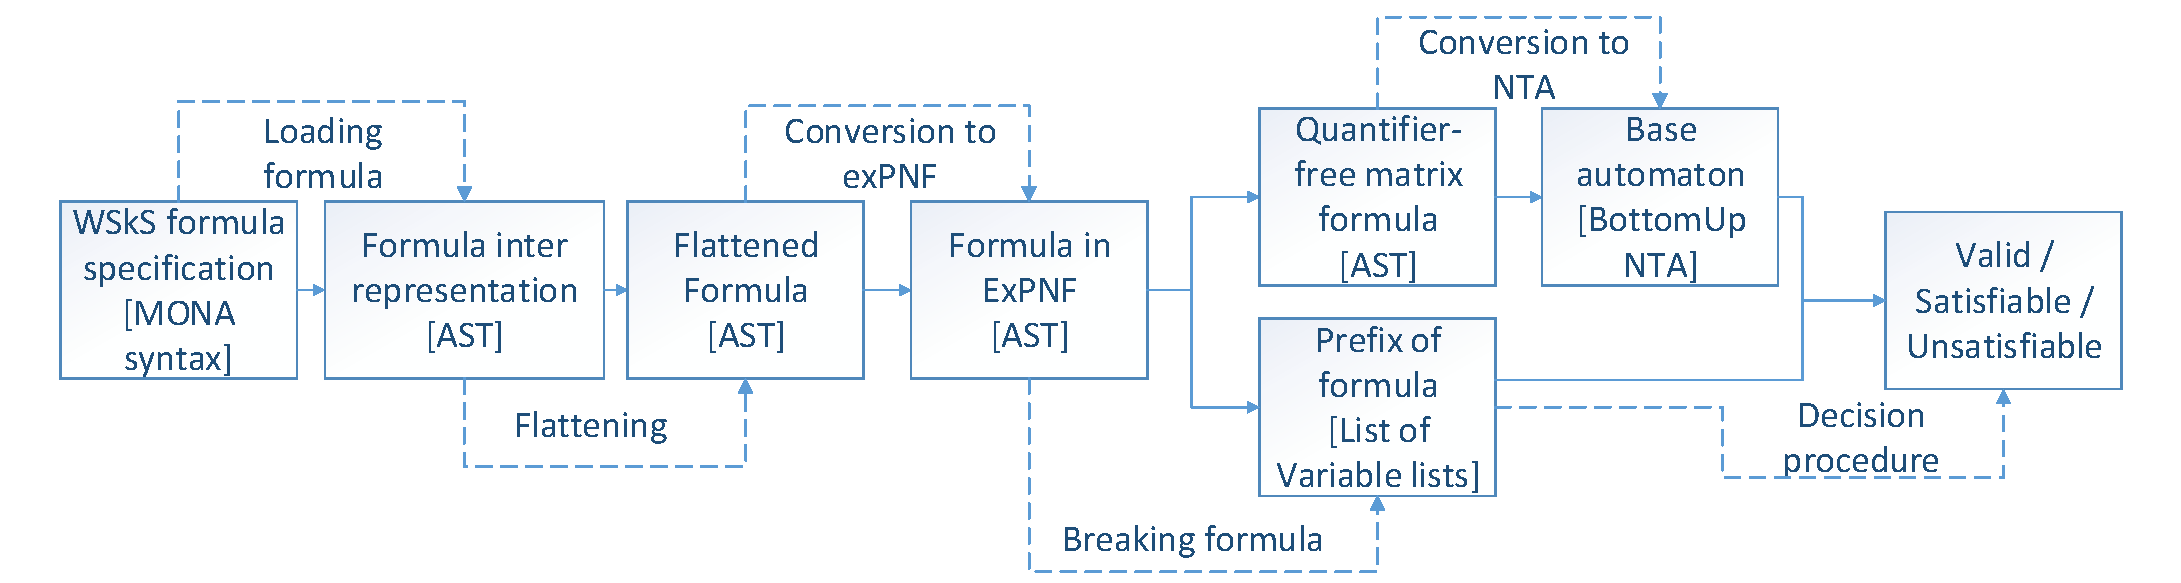
\includegraphics{fig/flow.pdf}}
 \caption{Transformation of data through the decision procedure}\label{flow}
 \end{center}
\end{figure}

\section{Manipulation with NTA}

For the inner representation of automata used in the decision procedure, the
\texttt{libvata} library \cite{vata-tool}, written in C++, was chosen for being
a highly efficient and open source library that exploits some of the recent
developments of algorithms for NTA manipulation. Its main use is in the fields
of formal verification, but it can be efficiently used in other domains as well.

\texttt{libvata} supports two possible encodings of tree automata
(\emph{explicit} and \emph{semi-symbolic}) which differ in the way they store
the transition relatios of automata. The semi-symbolic representation uses
MTBDDs for storing the transitions of automata as described in Section
\ref{mtbdd}. This is mostly intended for automata with large input alphabets
like in the case of some decision procedures of logics such as WS$k$S or MSO
\cite{mso} (monadic second-order logic). The library is designed in a modular
way, so it can be easily extended with new encodings and operations.

The library provides a command line interface, so the input of the library is
usually a text representation in automaton in Timbuk format \cite{timbuk}, which
is parsed and transformed into inner representation with states, transition,
alphabets, etc. However we can also build the automaton from scratch using API
functions for appropriate encodings. Each automaton can be serialized back to an
output format (like Timbuk) through serializers.

We are going to use the semi-symbolic encoding that provides both bottom-up and
top-down representation of tree automata. These representation differs in
storage of MTBDD where for top-down representation the storage is more complex,
while on the other hand, in the bottom-up representation arity can be inferred
from the arity of the tuples on the left-hand side of the transition.

As for the representation of automata, we have chosen the bottom-up
representation.

 \section{Decision procedure}
 
 In Chapter \ref{our} we introduced the formal concepts of deciding WS$k$S
 with non-deterministic automata and designed the algorithm for testing
 validity of a given formula $\varphi$. In this section we will closely describe
 the practical implementation of this formal algorithm in the C++ language.
 
 For each level $1 \leq i \leq m$ we define two caches that will store the
 already computed results to avoid their repeated computation during the
 decision procedure. In case we get a cache miss, the value $\bot$ is returned
 instead. $\mathit{BDDCache}_i$ is a cache that maps states of level $i$ to
 their corresponding MTBDDs representing their transition relations $\delta_i$, i.e.
 \begin{equation}
  \mathit{BDDCache} : Q_i \rightarrow ((\Sigma_i \rightarrow 2^{Q_i}) \cup
  \{\bot\}).
 \end{equation}
 
 Further we define the cache $\mathit{StateCache}_i$ for storing which states
 are final and which are non-final, i.e.
 \begin{equation}
  \mathit{StateCache} : Q_i \rightarrow \{Final, NonFinal, \bot\}
 \end{equation}
 
 The core function for deciding WS$k$S is \ref{impl-state-is-final} which checks
 whether there exists a reachable final state on level $0 \leq i \leq m$ from
 state $q$. This function is corresponding to the implementation of algorithm
 \ref{deciding-wsks-alg} with use of function \ref{impl-succ} for building successors of
 states and Algorithm \ref{impl-main} for checking whether the state is final.
 The implementation is using the workset algorithm and uses apply operations
 over the MTBDDs of constructed successors.
 
\begin{function}[h!]
		\SetKwFor{For}{foreach}{do}{}
		\SetKwRepeat{Repeat}{repeat}{until}
		\KwIn{State $q$ of automaton $A_{\varphi_m}$, level of determinization $m$}
		\KwOut{\textsc{TRUE} if there is reachable accepting state from $q$,
		\textsc{FALSE} otherwise}
		\BlankLine
		\nl workset := $\{q\}$\;
		\nl processed := workset\;
		\nl \While{$\exists q_m \in workset$}{
			\nl workset := workset $\setminus \{q_m\}$\;
			\nl\uIf{\upshape \texttt{IsStateFinal}($q_m$, $m$)}{
				\nl \Return \textsc{TRUE}\;
			}
			\nl\Else{
				\nl succ := \texttt{buildSuccessorTree($q_m$, m)}\;
				\nl\textbf{apply1} succ ($\lambda$ x. \textbf{if} $x \notin $processed$
				\wedge \not\exists y \in $processed$: x < y$ \textbf{then} workset :=
				workset $\cup \{x\}$)\; 
				\nl processed := processed $\cup$ workset\; 
				} 
			}
			\Return \textsc{FALSE}\;
		\caption{CheckForAcceptingState(state q, level m)}\label{impl-state-is-final}
\end{function}
 
 The main Algorithm \ref{impl-main} for deciding WS$k$S is corresponding to the
 implementation of Algorithm \ref{universality}. It first checks the cache
 whether the state has already been decided and else call the
 \ref{impl-state-is-final} function for checking for reachable final state. We
 can further extend this procedure to deciding satisfiability of WS$k$S
 formulae by checking the validity of $\exists$-closed input formulae. This
 means that given the input we close the formula and its negation and test the
 validity of constructed formulae to decide their satisfiability. Further we can
 decide the formula according to the relationships between validity,
 satisfiability and unsatisfiability.
 
\begin{algorithm}[h!]
		\SetKwFor{For}{foreach}{do}{}
		\SetKwRepeat{Repeat}{repeat}{until}
		\KwIn{State $I_m$ of automaton $A_{\varphi_m}$, level of determinization $m$}
		\KwOut{\textsc{TRUE} if state $I_m$ is final, \textsc{FALSE} otherwise}
		\KwData{\texttt{StateCache} caches the answers of \texttt{StateIsFinal}
		function}
		\BlankLine
		\nl\Return \texttt{IsStateFinal}($I_m$, $m$)\;
		\BlankLine
		\SetKwProg{myproc}{Function}{}{}
 		\myproc{\upshape \texttt{IsStateFinal}(\textbf{state} P, \textbf{level}
  i)}{ 
  		\nl isFinal := \texttt{StateCache}[P, m]\;
  		\nl\uIf{isFinal $\neq \bot$}{
  			\nl \Return isFinal\;
  		}
  		\BlankLine
  		\nl\uIf{m = 0}{
  		  \nl \Return $Q \in F_0$\;
  		}
  		\nl\Else{
  			\nl\For{$q \in Q$}{
  				\nl\uIf{\upshape \texttt{CheckForAcceptingState(q, m-1)}}{
  				    \nl \texttt{StateCache}[P, m] := \textsc{FALSE}\;
  					\nl\Return \textsc{FALSE}\;
  				}
  			}
  			\nl \texttt{StateCache}[P, m] := \textsc{TRUE}\;
  			\nl \Return \textsc{TRUE}\;
  		}
  }
		\caption{Implementation of deciding validity of WS$k$S formula
		}\label{impl-main}
	\end{algorithm}
 
 The successor of a state can be constructed out of its children
 as described by function \ref{impl-succ}.
 This construction is optimized with the use of cache. After the MTBDDs for
 transitions of children of a state are built, we use the binary apply for doing
 the union of those MTBDDs to yield the MTBDD corresponding to the transition
 from the state. This MTBDD is further modified using the operation of
 projection.
 
\begin{function}[h!]
		\SetKwFor{For}{foreach}{do}{}
		\SetKwRepeat{Repeat}{repeat}{until}
		\KwIn{State $q$ of automaton $A_{\varphi_m}$, level of determinization $m$}
		\KwOut{Successor of state $q$}
		\KwData{\texttt{BDDCache} mapping macro-states to their transition BDDs}
		\BlankLine
		\nl succ := \texttt{BDDCache}[q]\;
		\nl \uIf{succ $\neq \bot$}{
			\nl \Return succ\;
		}
		\nl succ := $\emptyset$\;
		\nl\For{$r \in q$}{
			\nl childSucc := \texttt{buildSuccessorTree(r, m-1)}\;
			\nl \textbf{apply2} succ childSucc ($\lambda$ x y. x $\cup$ y)\;
		}
		\nl succ := \texttt{project}(succ, level)\;
		\nl \texttt{BDDCache}[q] := succ\;
		\nl \Return succ\;
		\caption{buildSuccessorTree(state q, level m)}\label{impl-succ}
	\end{function}
 
 \section{Optimizations}
 
 During the implementation process we used the tool \texttt{valgrind}
 \cite{valgrind}, especially its part \texttt{callgrind}, to profile the
 implementation in C++ and tried to identify weak spots of the application.
 One of the most frequent operations in the procedure are the relational
 operators on the classes representing macro-states used e.g. for pruning the state search,
 macro-state comparison and operations with worklist.
 
 We propose to optimize this by using bitwise operations and bit array for
 storing the leaf states to ease some of the computation. There are several
 possibilities to use in C++ \cite{bitwise} and we have chosen the container
 with best performance, which is \texttt{boost::dynamic\_bitset}. The results
 have shown that the performance of comparison between macro-states of first
 level of detereminization got better by great margin.
 
 \subsection{Extending set of atomic formulae}
 
 While the set of atomic formulae in restricted syntax is indeed enough for
 defining whole range of WS$k$S logic, automata corresponding to the flattened
 versions of some of the atomic formulae (like $\leq$ for example) are too large
 for processing and slow down the algorithm. As shown in Table
 \ref{atomic-formulae} we can heavily reduce the size of matrix automaton just
 by extending the set of the atomic formulae defined in \ref{restricted} and
 construct special automata for frequently used operations and yielding smaller
 base automaton in result.
 
 \noindent\hrulefill
 \begin{example}
 Let us take $\varphi = x \leq y$ for example. In the classical restricted
 syntax, this formula $\varphi$ would be flattened as follows:
 \begin{equation}
  x \leq y \overset{\mathit{def}}{=} \forall X. (y \in X \wedge (\forall z. z1
  \in X \Rightarrow z \in X)) \Rightarrow x \in X
 \end{equation} 
 which corresponds to automaton with X states. However we can construct the
 following atomic automaton with 4 states only, which means we can save Y\% of
 the number of the states.
 \end{example}
 
 \noindent\hrulefill
 
 Besides defining automata for more of the WS$k$S syntax connectives and atomic
 formulae, we can extend the syntax even further and create some of the more
 complex operations like modulo or predecessor predicate, just like
 \textsc{MONA} does, that is not specifically defined in WS$k$S logic. 
 
 Note that we can decide Presburger formulae \cite{presburger} with basic set of
 automic formulae as shown for example in \cite{presburger-wsks}. This
 approach yields big automata in process one alternation of negation for each
 addition in formula. However we can construct a special automaton accepting the
 addition of two Presburger constants with 4 states only, thus greatly reducing
 the time needed to decide this formula.
 
 \subsection{Cache}
 
 The caching of some of the already computed results can be applied to several
 places in code. First we can cache the already computed answers for finality of
 macro-states. Second during the computation of successors of states, we can
 cache the BDDs that were already constructed before.
 
 With the design of algorithm, which is looking for existing example, i.e.
 searching for reachable state, in automaton corresponding to the formulae and
 its negation (to get counterexample) this means we don't have to compute
 and classify lots of states twice.
 
 {\color{red} Here will be several evaluations of ratio between cache hits and
 misses.}

\chapter{Evaluation}

In this chapter we are going to provide an evaluation of the implemented
decision procedure described in the previous chapters. The performance was
tested on two different scenarios and compared with the implementation of the
procedure using deterministic tree automata \textsc{MONA}. The first batch of
tests measures how our implementation resulted in terms of quantification and
how more quantifiers adds to the computational speed-up. The other tests are
evaluating decision of quantifier free formulae. 

\iffalse
\section{Presburger Arithmetic}

One of the classical logics is Presburger Arithmetic \cite{pres}, the
first-order theory of integer number with addition and ordering, which is
decidable. There exists an algorithm that can decide the Presburger formula in
$2^{2^{2^{pn\log n}}}$ time \cite{pres-time}. 

The WS$k$S is stronger logic and can be used for deciding of Presburger as well
by converting the formulae into WS$k$S and then use the described algorithm.
However this does not provide the faster algorithm as the bound complexity of
WS$k$S is higher than for Presburger Arithmetic. 

In Presburger Arithmetic a \texttt{term} is either a integer constant or a
variable. The Presburger formula is then either in form of $term < term$, $term
+ term$ or $constant * term$. It can be further assumed that the multipliers
are the powers of two.

The conversion to WS$k$S treats the variable as set with a set variable being a
bit of the binary representation of the number with addition of a sign bit.

The main convenience of these family of formulae that every operation $+$ or $*$
in a term generates at least one quantifier in the WS$k$S formulae, which can
further results to quite a large exponential blowup and hence show the speed-up
of our approach in contrary to the \texttt{MONA}.

The other parametric part of the presburger arithmetic is bounding of the
maximal constant used in expressions. Since constants are represented by sets
containing positions of ones in bit-wise representation of the constant, we can
further study the impact of this on performance of decision procedure.

So the formula $\varphi \overset{\mathit{def}}{=} X = \mathtt{pconst}{I}$, where
X is second-order variable representing constant $I$, as follows:
\begin{equation}
 \varphi \overset{\mathit{def}}{=} \bigwedge_{i = 0}^{\lceil \log_2 I\rceil} C_i
\end{equation}
where
\begin{equation}
  C_i = \begin{dcases*}
         i \in X  & when $i$th bit of $I$ is set\\
         i \notin X & when $i$th bit of $I$ is not set
         \end{dcases*}
\end{equation}
with special case
\begin{equation}
  C_0 = \begin{dcases*}
          0 \in X  & if $I < 0$\\
         0 \notin X & if $I > 0$\\
         true & otherwise
         \end{dcases*}
\end{equation}

Further we can construct the formulae for operations of addition, relation
less-than and times 2 operation as follows:
\begin{eqnarray}
 plus(R, P, Q) & \overset{\mathit{def}}{=} & \exists Carry:
 noCarryIn(Carry) \wedge \forall t:\\
 &  propagateCarry(t, Carry, P, Q) & \wedge computeResults(t,
 Carry, P, Q, R)\\
 less(P, Q) & \overset{\mathit{def}}{=} &\exists R: T \neq \{\empty\} \wedge
 plus(Q, P, T)\\
 timesTwo(P, Q) & \overset{\mathit{def}}{=} & plus(Q, P, P) 
\end{eqnarray}
where
\begin{eqnarray}
 propagateCarry(Carry, P, Q) & \overset{\mathit{def}}{=} & t + 1 \in Carry
 \Leftrightarrow at_least_two(t \in P, t \in Q, t \in Carry)\\
 computeResult(t, Carry, P, Q, R) & \overset{\mathit{def}}{=} & t \in R
 \Leftrightarrow xor(xor(t \in P, t \in Q), t \in Carry)\\
 at_least_two(\varphi_1, \varphi_2, \varphi_3) & \overset{\mathit{def}}{=} &
 (\varphi_1 \wedge \varphi_2) \vee (\varphi_1 \wedge \varphi_3) \vee (\varphi_2
 \wedge \varphi_3)\\
 xor(\varphi_1, \varphi_2) & \overset{\mathit{def}}{=} & (\varphi_1 \wedge
 \neg\varphi_2) \vee (\neg\varphi_1 \wedge \varphi_2)
\end{eqnarray}

Random formulae were generated with different number of quantifiers and bounded
by different constants and evaluated by both \texttt{MONA} and our tool. 

\fi

\section{Parametric horn formulae}

Other experiments done with our implemented tool were carried out on specific
artificially created parametric formulae in Horn form \cite{horn}. 

\begin{defz}
We a formula $\varphi$ a \emph{Horn formula} if\ldots
\end{defz}

The concrete formula with parameter $n$ is in form of
\begin{equation}
 \varphi_n \overset{\mathit{def}}{=} \exists X\forall x_1\ldots x_n.
 \bigwedge_{i = 1}^{n-1} (x_i \in X \Rightarrow x_{i+1} \in X)
\end{equation}

This family of formulae is valid. It was further examined that \textsc{MONA} can
only decide the formulae up to parameter $n = 15$ due to insufficient memory for
storing BDDs. In results it is shown that the logical approach
\cite{logic-approach} proves to better for solving this family of formulae in
contrary to automata-formulae connection used by both \textsc{MONA} and our approach.

\chapter{Conclusion}\label{summary}

In this work we introduced the WS$k$S logic and some its decision procedures. We
have described the classical approach that uses deterministic automata, as well
as tool \textsc{MONA} that enhances this procedure by using several optimizations and
discussed their complexity issues and problems they have to deal with.

Another approach was proposed that uses non-deterministic automata instead of
deterministic ones. This makes use of recent developments in fields of
non-deterministic automata algorithms, like universality checking or language
inclusion, allowing us to implement procedure similar to anti-chain based
testing \cite{tacas} and search for rejecting or accepting states on-the-fly
without need to construct automaton corresponding to the given formula at all.

We implemented a prototype of the designed decision procedure, that is able to
handle a subset of WS$k$S formulae, namely formulae for case $k = 1$, and
studied the impact of the usage of non-deterministic automata on two case
studies. Out of the computational results on series of formulae we identified
some of the weak spots of the application and tried to optimized them to achieve
better results.

Although our results could not beat \textsc{MONA} and its many heuristics and
optimizations, we have shown that the non-deterministic approach to deciding
WS$k$S has indeed great potential and yield good results with future research.

Just like \textsc{MONA} did, we propose some further optimizations that could
enhance the results in processes. One of the weak spots of algorithm is the size
of the base automaton corresponding to the unquantified part of the formula.
\textsc{MONA} always does minimization after every operation so it works with
the smallest automata possible. We can reduce the size of non-deterministic
automata through simulation computation followed by downward reduction. 

Most of the formulae used in practice share very similar subformulae that can be
represented as single node and reuse the constructed automaton by reindexing its
variables. We propose to optimize the frontend of the procedure to use the
Direct Acyclic Graph (DAG) instead of plain AST. 

%=========================================================================
